\def\theory{
    \section{Cơ sở lý thuyết}
    Các nghiên cứu hiện đại nhất về việc giải quyết bài toán nhận diện khuôn mặt và nhận diện khuôn mặt trong ảnh chất lượng cao kế thừa rất nhiều ý tưởng từ các nghiên cứu giải quyết bài toán nhận diện đối tượng \index{nhận diện đối tượng}.

    \noindent
    Các mô hình giải quyết bài toán nhận diện đối tượng \index{nhận diện đối tượng} được chia thành hai nhóm: nhóm các mô hình hai pha \index{hai pha} (two-stage) và nhóm các mô hình một pha \index{một pha} (single-stage).
    Các mô hình hai pha \index{hai pha} phổ biến là R-CNN \cite{girshick2014rich}, Fast R-CNN \cite{girshick2015fast}, Faster R-CNN \cite{ren2015faster} và FPN \cite{lin2017feature}.
    Các mô hình hai pha \index{hai pha} này đạt độ chính xác rất cao, tuy nhiên, tốc độ chạy không thật sự nhanh và đây là động lực để các mô hình một pha \index{một pha} ra đời. 
    Các mô hình một pha \index{một pha} nổi tiếng và thu hút nhiều sự quan tâm như SSD \index{SSD} \cite{liu2016ssd}, chuỗi các mô hình YOLO \index{YOLO} \cite{redmon2016look, redmon2016yolo9000, redmon2018yolov3, bochkovskiy2020yolov4}, RetinaNet \cite{lin2017focal}.

    \noindent
    Bên cạnh đó, nhiều nghiên cứu trong những năm gần đây đã tập trung vào việc xử lý ảnh chất lượng cao.
    Các mô hình này hướng tới việc duy trì và tăng cường độ chính xác của mô hình nhận diện đối tượng \index{nhận diện đối tượng} và tiết kiệm tối đa chi phí tính toán.
    Một số nghiên cứu đáng chú ý như SNIP \cite{singh2018analysis}, SNIPER \index{SNIPER} \cite{singh2018sniper}, Scale Match \cite{yu2020scale} hướng đến quá trình huấn luyện của mô hình với ảnh chất lượng cao, AutoFocus \index{AutoFocus} \cite{najibi2019autofocus}, Attention pipeline \cite{ruuvzivcka2018fast}, Dynamic Zoom-in \cite{gao2018dynamic}, PeleeNet \cite{ozge2019power} đưa ra các ý tưởng cải thiện quá trình dự đoán của mô hình với ảnh chất lượng cao.

    \noindent
    Lấy nền tảng từ các mô hình nhận diện đối tượng \index{nhận diện đối tượng}, các mô hình nhận diện khuôn mặt bổ sung hoặc chỉnh sửa một số điểm nhằm tăng độ chính xác trên các bộ dữ liệu về khuôn mặt.
    Dựa trên SSD \index{SSD} \cite{Liu_2016}, mô hình S3FD \cite{zhang2017s3fd} thay đổi chiến lược sinh anchor \index{anchor} nhằm đạt độ chính xác cao hơn trên dữ liệu khuôn mặt.
    Mô hình Pyramid Box \cite{tang2018pyramidbox} và Pyramid Box++ \cite{li2019pyramidbox++} thay đổi kiến trúc của mô hình FPN \cite{lin2017feature} phù hợp hơn đối với bài toán nhận diện khuôn mặt.
    Hay mô hình RetinaFace \cite{deng2020retinaface}, kế thừa từ RetinaNet \cite{lin2017focal}, sử dụng thêm dữ liệu và hàm mất mát đặc trưng của khuôn mặt.

    \subsection{Mô hình Faster R-CNN}
    \def\fasterrcnn{
    Được lấy động lực từ những điểm yếu của mô hình Fast R-CNN \cite{girshick2015fast}, nhóm tác giả đã nghiên cứu và phát triển mô hình Faster R-CNN \cite{ren2015faster} với trung tâm là kiến trúc mô hình Region Proposal Network (gọi tắt là RPN).
    Mô hình Region Proposal Network được kỳ vọng sẽ thay thế hoàn toàn các thuật toán như Selective Search \cite{uijlings2013selective} trong thành phần region proposals module \index{region proposals module} của các mô hình two-stage giải quyết bài toán object detection, hướng đến việc cải thiện không chỉ tốc độ của mô hình mà còn cải thiện về độ chính xác.

    \subsubsection{Kiến trúc mô hình Region Proposal Network}
    Mô hình RPN nhận đầu vào là ảnh với kích thước bất kỳ và trả đầu ra là toạ độ của các khu vực và xác suất khu vực đó là đối tượng nào trong các lớp đối tượng \index{lớp đối tượng}.
    Nhằm tiết kiệm chi phí tính toán, mô hình RPN dùng chung phần feature extraction module \index{feature extraction module} với Fast R-CNN.

    \begin{figure}[H]
        \centering
        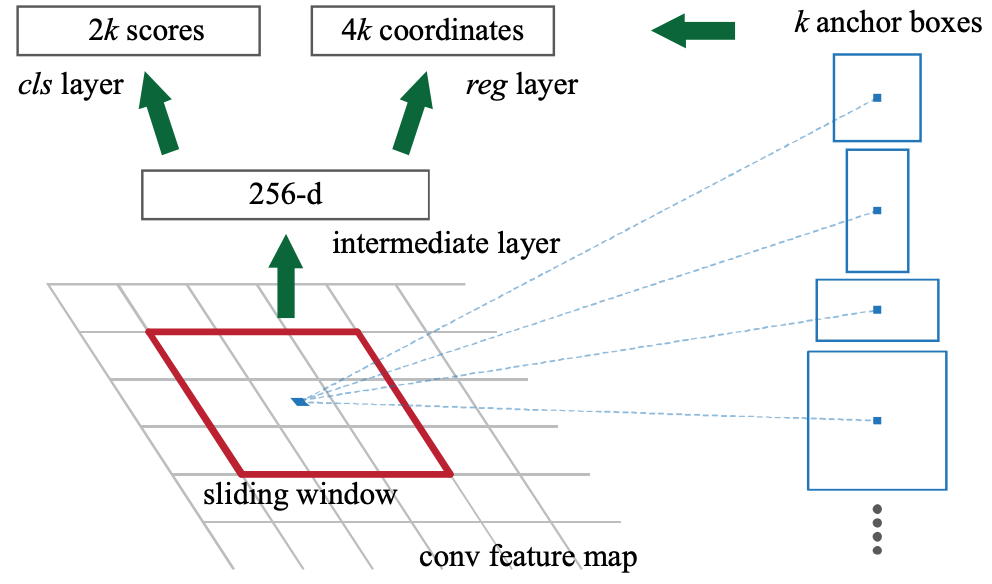
\includegraphics[width=9cm] {images/faster_rcnn_rpn}
        \caption{Kiến trúc mô hình Region Proposal Network (Nguồn: \cite{ren2015faster})}
        \label{fig:faster_rcnn_rpn}
    \end{figure}
    
    \noindent
    Sau khi đưa ảnh qua feature extraction module \index{feature extraction module} và thu được một feature maps, mô hình RPN nhận đầu vào là feature maps \index{feature maps} này và trả đầu ra là các khu vực đề xuất gọi là các anchor \index{anchor}.
    Nhóm tác giả xây dựng phương pháp đề xuất các anchor \index{anchor} dựa trên kích thước và tỷ lệ giữa chiều dài và chiều rộng của anchor \index{anchor}.
    Cụ thể, mô hình RPN đưa feature maps \index{feature maps} qua một lớp Conv \index{lớp Conv} và thu được một feature maps \index{feature maps} mới có kích thước $W x H$.
    Từ đó, nhóm tác giả đề xuất ba kích thước của anchor \index{anchor} và ba tỷ lệ giữa chiều dài và chiều rộng của anchor \index{anchor} tạo ra chín anchor \index{anchor} với mỗi pixels \index{pixels} trên feature maps \index{feature maps} kích thước $W x H$.
    Tổng cộng trên toàn bộ feature maps \index{feature maps} kích thước $W x H$, ta thu được $W x H x 9$ anchor \index{anchor}.
    Các feature maps \index{feature maps} đại diện cho các anchor \index{anchor} này được tiếp tục đưa qua các lớp Conv \index{lớp Conv} để biến đổi về các feature maps \index{feature maps} mới có dạng $(W x H x 9) x 1$ đại diện cho xác suất anchor \index{anchor} đó là object và có dạng $(W x H x 9) x 4$ đại diện cho 4 toạ độ x của góc trái trên, y của góc trái trên, chiều dài và chiều rộng của bounding box \index{bounding box}.

    \noindent
    Một điểm mạnh của RPN so với các mô hình object detection thời bấy giờ đó chính là khả năng dự đoán được các object có kích thước khác nhau và tỷ lệ giữa chiều dài và chiều rộng khác nhau nhờ vào cách cấu hình của anchor \index{anchor}.

    \begin{figure}[H]
        \centering
        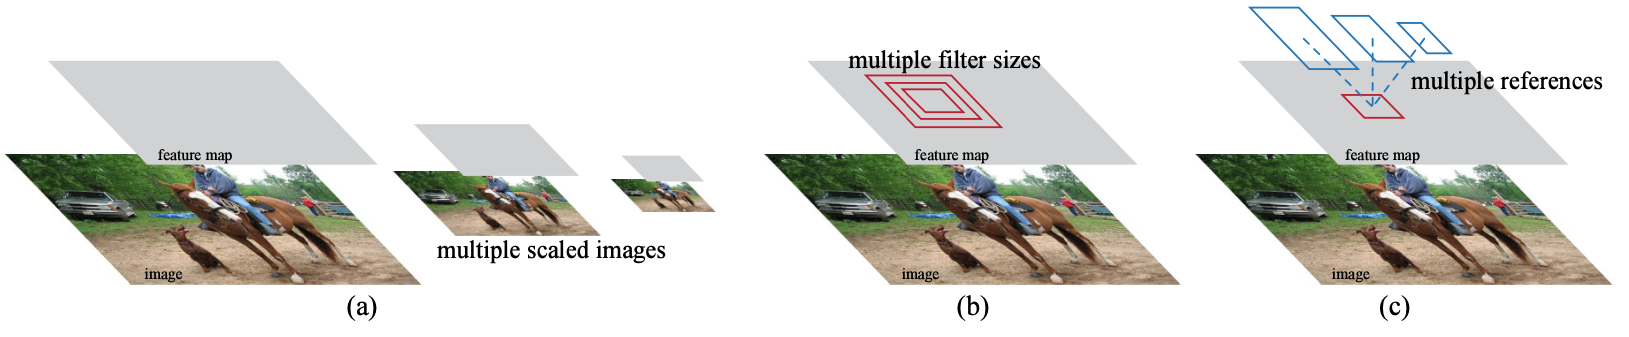
\includegraphics[width=15cm] {images/faster_rcnn_multi_scale_anchor}
        \caption{So sánh các kiến trúc xử lý vấn đề object có kích thước khác nhau và tỷ lệ giữa chiều dài và chiều rộng khác nhau (Nguồn: \cite{ren2015faster})}
        \label{fig:faster_rcnn_multi_scale_anchor}
    \end{figure}

    \noindent
    Một số kiến trúc đã được đề xuất ở thời điểm đó nhưng đều gặp phải rào cản về khối lượng tính toán lớn. \\
    - Kiến trúc đầu tiên là \textit{image/feature pyramids} sử dụng ảnh với nhiều kích thước khác nhau nhằm tạo ra feature maps \index{feature maps} có nhiều kích thước khác nhau.
    Kiến trúc này tốn rất nhiều chi phí tính toán do ta cần xử lý nhiều lần (thường là ba lần) với mỗi ảnh đầu vào khác nhau. \\
    - Kiến trúc thứ hai là \textit{pyramid of filters} đưa cùng một feature maps \index{feature maps} đầu vào qua nhiều khối Conv có kích thước của kernel khác nhau (thường là Conv với kernel 5x7 và Conv với kernel 7x5).
    Kiến trúc này tiết kiệm chi phí tính toán hơn một chút so với kiến trúc đầu tiên và thường được sử dụng kết hợp cùng với kiến trúc đầu tiên. \\
    - Kiến trúc cuối cùng là \textit{pyramid of anchors} được đề xuất trong RPN sử dụng nhiều anchor \index{anchor} với các kích thước khác nhau và tỷ lệ giữa chiều dài và chiều rộng khác nhau.
    Kiến trúc này chỉ tăng một lượng nhỏ chi phí tính toán nếu ta tăng số lượng anchor \index{anchor}, còn phần chi phí tính toán đối với feature maps \index{feature maps} vẫn được giữ nguyên. \\
    Phần cải tiến của RPN đối với object có kích thước khác nhau và tỷ lệ giữa chiều dài và chiều rộng khác nhau chỉ là những cải tiến tại thời điểm đó mà thôi.

    \subsubsection{Hàm loss và cách huấn luyện mô hình RPN}
    Để huấn luyện được mô hình RPN, nhóm tác giả gán cho mỗi anchor \index{anchor} một lớp groundtruth \index{groundtruth} và thiết lập hàm loss đối với từng anchor \index{anchor}.
    Nhóm tác giả gán lớp groundtruth \index{groundtruth} positive cho anchor \index{anchor} dựa theo hai cách sau: \\
    - Những anchor \index{anchor} có chỉ số IoU \index{IoU} lớn nhất đối với một groundtruth \index{groundtruth} bounding box \index{bounding box} được gán là anchor \index{anchor} positive. \\
    - Những anchor \index{anchor} có chỉ số IoU \index{IoU} lớn hơn 0.7 đối với một groundtruth \index{groundtruth} bounding box \index{bounding box} được gán là anchor \index{anchor} positive. \\
    Với hai cách như trên, một groundtruth \index{groundtruth} bounding box \index{bounding box} có thể gán được cho nhiều anchor \index{anchor} khác nhau.
    Ngoài ra, nhóm tác giả cũng gán lớp groundtruth \index{groundtruth} negative cho các anchor \index{anchor} không phải là positive và có chỉ số IoU \index{IoU} nhỏ hơn 0.3 đối với một groundtruth \index{groundtruth} bounding box \index{bounding box}. \\
    Từ đó, mô hình Faster R-CNN tối ưu hàm loss sau:

    \begin{equation}
        \label{eq:faster_rcnn_loss}
        L(\{p_i\}, \{t_i\}) = \frac{1}{N_{cls}}\sum_i L_{cls}(p_i, p^{*}_i) + \lambda\frac{1}{N_{reg}}\sum_i  p^{*}_i L_{reg}(t_i, t^{*}_i).
    \end{equation}

    \noindent
    trong đó: \\
    - \textit{i} là chỉ số của từng anchor \index{anchor}. \\
    - \textit{$p_i$} là xác suất mà anchor \index{anchor} chứa đối tượng. \\
    - \textit{$p^{*}_i$} là groundtruth \index{groundtruth} của anchor \index{anchor} (là 1 nếu anchor \index{anchor} đó được gán là chứa đối tượng, là 0 nếu anchor \index{anchor} đó được gán là không chứa đối tượng). \\
    - \textit{$t_i$} là vector gồm 4 giá trị đại diện cho toạ độ của khu vực mà mô hình RPN đề xuất. \\
    - \textit{$t^{*}_i$} là vector gồm 4 giá trị đại diện cho toạ độ của groundtruth \index{groundtruth} bounding box \index{bounding box} tương ứng với anchor \index{anchor} đó. \\
    Hàm loss trên gồm các thành phần: \\
    - \textit{$L_{cls}$}: là hàm loss phân lớp thông thường giúp xác định anchor \index{anchor} có chứa đối tượng hay không. \\
    - \textit{$L_{reg}$}: là hàm loss hồi quy đối với các anchor \index{anchor} positive, giúp tinh chỉnh toạ độ của khu vực mà mô hình đề xuất.
    Cụ thể, nhóm tác giả sử dụng $L_{reg}(t_i, t^{*}_i)=L_1(t_i - t^{*}_i)$ giống với hàm loss sử dụng trong mô hình Fast R-CNN \cite{girshick2015fast}.

    \noindent
    Mô hình RPN được thiết kế để có thể huấn luyện cùng với quá trình huấn luyện object detection từ đó giúp kết quả đề xuất khu vực trở nên chính xác hơn.
    Tuy nhiên, có một vấn đề nảy sinh khi sử dụng mô hình RPN cho việc đề xuất khu vực, đó là mô hình sẽ đề xuất ra nhiều các anchor \index{anchor} negative hơn rất nhiều so với số anchor \index{anchor} positive.
    Việc huấn luyện mô hình trên từng anchor \index{anchor} kết hợp với hiện tượng trên sẽ khiến cho tổng quan mô hình object detection bị mất cân bằng dữ liệu \index{mất cân bằng dữ liệu}.
    Ngoài ra, việc huấn luyện mô hình với toàn bộ số anchor \index{anchor} được đề xuất ra cũng sẽ khiến cho khối lượng tính toán lớn và thời gian kéo dài quá trình huấn luyện mô hình.
    Từ đó, nhóm tác giả đề xuất việc lựa chọn ngẫu nhiên 256 anchor \index{anchor} trên mỗi ảnh để thực hiện việc tính loss. Việc lựa chọn này giúp tỷ lệ anchor \index{anchor} positive và negative trở nên cân bằng hơn và giảm thiểu bởi những phần khối lượng tính toán dư thừa.

    \noindent
    \textbf{\textit{Sự kết hợp giữa mô hình Region Proposal Network và Fast R-CNN}} \\
    Nhóm tác giả cho rằng, việc huấn luyện mô hình RPN và Fast R-CNN cần phải diễn ra đồng thời, vì từ đó, việc chia sẻ chung thành phần backbone Conv mới trở nên hiệu quả.

    \begin{figure}[H]
        \centering
        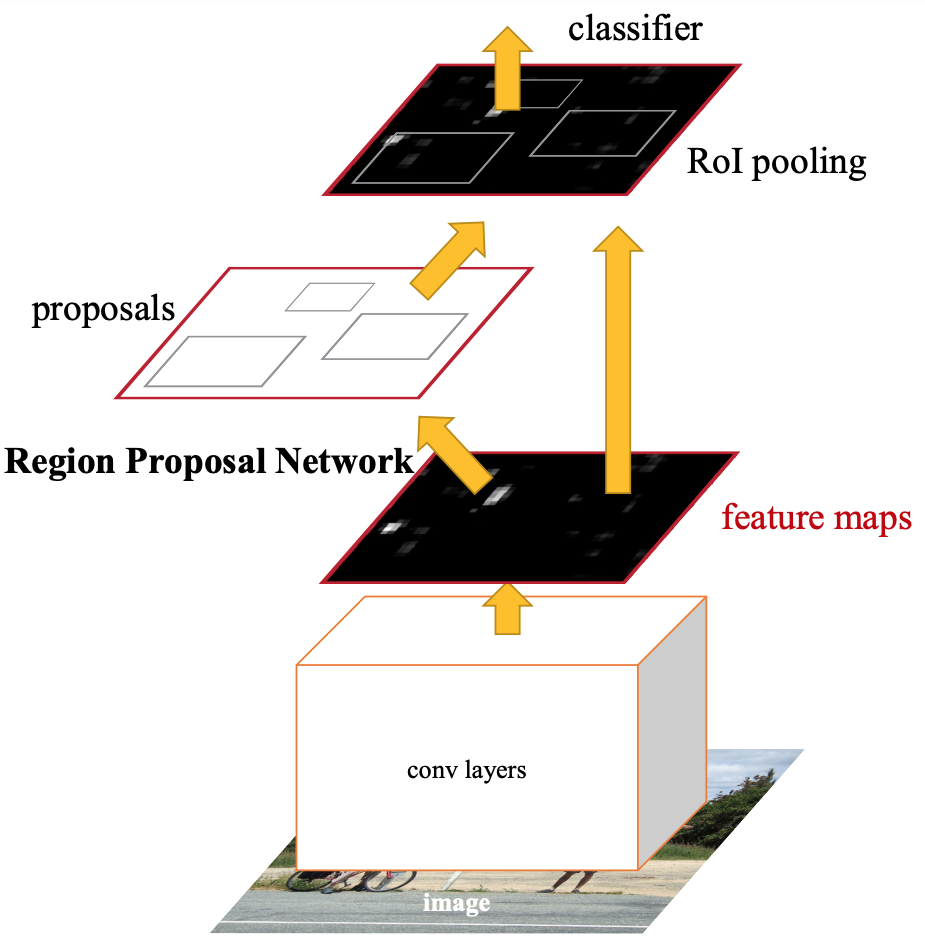
\includegraphics[width=10cm] {images/faster_rcnn_model}
        \caption{Toàn cảnh sự kết hợp của mô hình Region Proposal Network và Fast R-CNN tạo ra mô hình Faster R-CNN (Nguồn: \cite{ren2015faster})}
        \label{fig:faster_model}
    \end{figure}

    \noindent
    Nhóm tác giả nêu ra ba phương án để huấn luyện mô hình RPN kết hợp với Fast R-CNN: \\
    - Cách 1: \textit{Alternating training}: Nhóm tác giả huấn luyện mô hình RPN trước sử dụng những hàm loss của RPN nói trên.
    Sau khi huấn luyện xong mô hình RPN, tác giả sử dụng những khu vực được đề xuất bởi RPN để huấn luyện mô hình Fast R-CNN.
    Mô hình backbone sau khi được huấn luyện bởi Fast R-CNN tiếp tục được sử dụng để huấn luyện mô hình RPN mới và vòng lặp này tiếp tục diễn ra cho đến khi kết quả của mô hình hội tụ. \\
    - Cách 2: \textit{Approximate joint training}: Phương pháp này kết hợp RPN và Fast R-CNN thành một mô hình duy nhất trong quá trình huấn luyện.
    Các khu vực được đề xuất bởi RPN được coi như là tất định đối với nhánh Fast R-CNN và khiến cho phương pháp huấn luyện này được gọi là \textit{approximate} bởi vì những thông tin từ nhánh Fast R-CNN sẽ không được cập nhật cho nhánh RPN.
    Quá trình backprop được thực hiện độc lập giữa RPN và Fast R-CNN, riêng phần backbone chung của RPN và Fast R-CNN được cập nhật theo giá trị hàm loss của cả RPN và Fast R-CNN.
    Phương pháp này đạt hiệu quả thấp hơn chút so với \textit{Alternating training} tuy nhiên thời gian huấn luyện được giảm 25 - 50\%. \\
    - Cách 3: \textit{Non-approximate joint training}: Phương pháp này cải thiện được vấn đề \textit{approximate} tồn đọng của \textit{Approximate joint training}.
    Tuy nhiên, để làm được điều này, nhóm tác giả cần tinh chỉnh lại lớp RoI pooling trong Fast R-CNN để có thể update cho cả các thành phần của mô hình Fast R-CNN và RPN.
    Điều này nằm ngoài nội dung của nghiên cứu này nên nhóm tác giả không đề cập kỹ hơn.

    \noindent
    Tóm lại, nhóm tác giả dựa vào phương pháp \textit{Alternating training} và thực hiện quá trình huấn luyện gồm 4 bước như sau: \\
    - Bước 1: Nhóm tác giả khởi tạo mô hình RPN với pretrained ImageNet và huấn luyện mô hình RPN. \\
    - Bước 2: Nhóm tác giả khởi tạo mô hình Fast R-CNN với pretrained ImageNet và huấn luyện mô hình Fast R-CNN với các khu vực được đề xuất bởi RPN. \\
    - Bước 3: Nhóm tác giả khởi tạo lại mô hình RPN nhưng sử dụng phần backbone đã được huấn luyện từ bước 2.
    Nhóm tác giả chỉ huấn luyện những lớp riêng của mô hình RPN và không cập nhật cho phần backbone. \\
    - Bước 4: Nhóm tác giả finetune lại những lớp riêng của mô hình Fast R-CNN với các khu vực được đề xuất bởi RPN và thu được mô hình Faster R-CNN cuối cùng. \\
    Nhóm tác giả cũng đã lặp lại 4 bước trên vài lần nhưng kết quả không thay đổi quá nhiều.

    % \noindent
    % \textbf{\textit{Kết quả của mô hình Faster R-CNN}} \\
    % Đầu tiên, trong hình \ref{fig:faster_rcnn_results_1}, kết quả của mô hình Fast R-CNN sử dụng RPN, backbone ZF-Net và dùng chung backbone giữa nhánh RPN và nhánh Fast R-CNN (\textbf{RPN+ZF, shared}) tốt hơn trên chỉ số mAP so sánh với việc sử dụng thuật toán Selective Search \textbf{SS} và EdgeBoxes \textbf{EB} trên bộ dữ liệu VOC 2007 test. Trong đó, số lượng khu vực được đề xuất trong quá trình huấn luyện được thống kê tại cột \textbf{\# boxes}, trong quá trình test được thống kê tại cột \textbf{\# proposals}.

    % \begin{figure}[H]
    %     \centering
    %     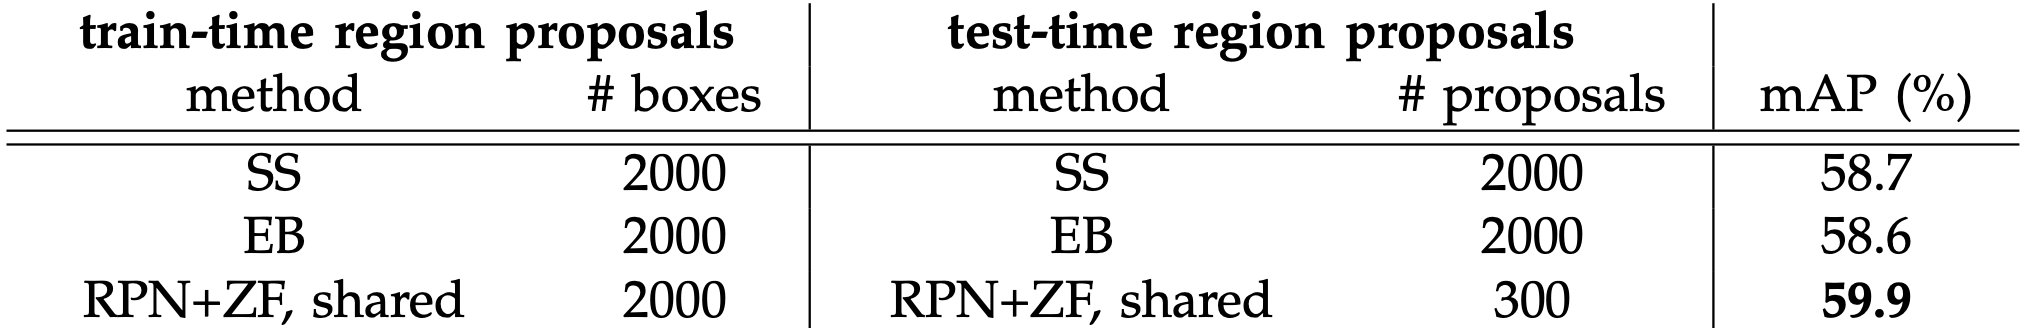
\includegraphics[width=10cm] {images/faster_rcnn_results_1}
    %     \caption{Kết quả của mô hình Fast R-CNN sử dụng RPN so sánh với việc sử dụng thuật toán Selective Search và EdgeBoxes trên bộ dữ liệu VOC 2007 test. (Nguồn: \cite{ren2015faster})}
    %     \label{fig:faster_rcnn_results_1}
    % \end{figure}

    % \noindent
    % Tiếp theo, trong hình \ref{fig:faster_rcnn_results_2}, nhóm tác giả so sánh kết quả của các mô hình Faster R-CNN (dùng backbone là VGG-16, ký hiệu là \textbf{RPN + VGG}) với mô hình Fast R-CNN sử dụng thuật toán Selective Search trên bộ dữ liệu VOC 2007 test nhưng với các bộ dữ liệu huấn luyện khác nhau. \\
    % - Cấu hình sử dụng riêng hai backbone khác nhau giữa nhánh RPN và nhánh Fast R-CNN: ký hiệu là \textbf{unshared} \\
    % - Cấu hình sử dụng chung backbone giữa nhánh RPN và nhánh Fast R-CNN: ký hiệu là \textbf{shared} \\
    % - Cấu hình sử dụng bộ dữ liệu huấn luyện là VOC07 trainval: ký hiệu là \textbf{07} \\
    % - Cấu hình sử dụng bộ dữ liệu huấn luyện là sự kết hợp giữa VOC07 trainval và VOC12 trainval: ký hiệu là \textbf{07+12} \\
    % - Cấu hình sử dụng bộ dữ liệu huấn luyện là sự kết hợp giữa VOC07 trainval, VOC12 trainval và bộ dữ liệu MS-COCO: ký hiệu là \textbf{COCO+07+12} \\
    % Trong đó, số lượng khu vực được đề xuất trong quá trình test được thống kê tại cột \textbf{\# proposals}. \\
    % Kết quả mô hình \textbf{RPN + VGG, unshared, 07} đạt chỉ số mAP là 68.5\%, tốt hơn so với 66.9\% của mô hình \textbf{SS, 07}.
    % Kết quả mô hình \textbf{RPN + VGG, shared, 07+12} đạt chỉ số mAP là 73.2\%, tốt hơn so với 70.0\% của mô hình \textbf{SS, 07+12}.
    % Và mô hình \textbf{RPN + VGG, shared, COCO+07+12} đạt chỉ số mAP cao nhất là 78.8\%, điều này khá dễ hiểu khi mô hình sử dụng nhiều dữ liệu huấn luyện hơn sẽ cho kết quả tốt hơn.

    % \begin{figure}[H]
    %     \centering
    %     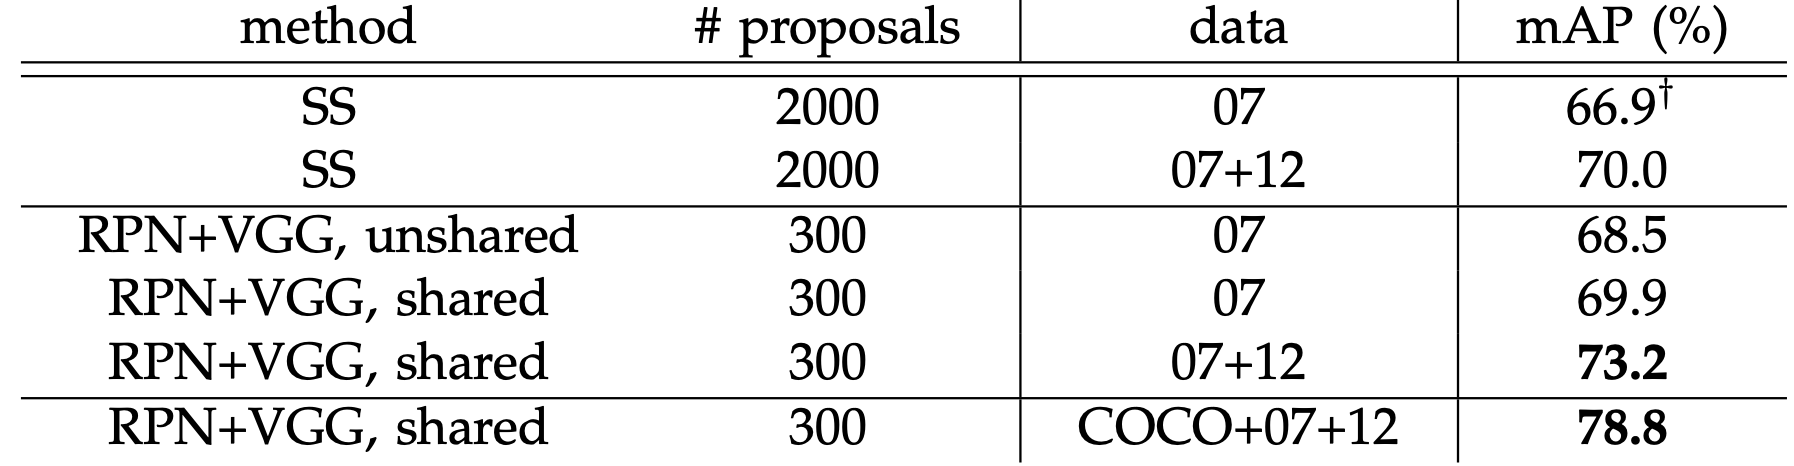
\includegraphics[width=10cm] {images/faster_rcnn_results_2}
    %     \caption{Kết quả của mô hình Fast R-CNN sử dụng RPN và backbone VGG-16 so sánh với mô hình Fast R-CNN sử dụng thuật toán Selective Search trên bộ dữ liệu VOC 2007 test với các bộ dữ liệu huấn luyện khác nhau. (Nguồn: \cite{ren2015faster})}
    %     \label{fig:faster_rcnn_results_2}
    % \end{figure}

    % \noindent
    % Tiếp theo, trong hình \ref{fig:faster_rcnn_results_3}, nhóm tác giả so sánh kết quả của các mô hình Faster R-CNN (dùng backbone là VGG-16, ký hiệu là \textbf{RPN + VGG}) với mô hình Fast R-CNN sử dụng thuật toán Selective Search trên bộ dữ liệu VOC 2012 test nhưng với các bộ dữ liệu huấn luyện khác nhau. \\
    % - Cấu hình sử dụng chung backbone giữa nhánh RPN và nhánh Fast R-CNN: ký hiệu là \textbf{shared} \\
    % - Cấu hình sử dụng bộ dữ liệu huấn luyện là VOC12 trainval: ký hiệu là \textbf{12} \\
    % - Cấu hình sử dụng bộ dữ liệu huấn luyện là sự kết hợp giữa VOC07 trainval+test và VOC12 trainval: ký hiệu là \textbf{07++12} \\
    % - Cấu hình sử dụng bộ dữ liệu huấn luyện là sự kết hợp giữa VOC07 trainval+test, VOC12 trainval và bộ dữ liệu MS-COCO: ký hiệu là \textbf{COCO+07+12} \\
    % Trong đó, số lượng khu vực được đề xuất trong quá trình test được thống kê tại cột \textbf{\# proposals}. \\
    % Kết quả mô hình \textbf{RPN + VGG, shared, 12} đạt chỉ số mAP là 67.0\%, tốt hơn so với 65.7\% của mô hình \textbf{SS, 12}.
    % Kết quả mô hình \textbf{RPN + VGG, shared, 07++12} đạt chỉ số mAP là 70.4\%, tốt hơn so với 68.4\% của mô hình \textbf{SS, 07++12}.
    % Và mô hình \textbf{RPN + VGG, shared, COCO+07++12} đạt chỉ số mAP cao nhất là 75.9\%, điều này khá dễ hiểu khi mô hình sử dụng nhiều dữ liệu huấn luyện hơn sẽ cho kết quả tốt hơn.

    % \begin{figure}[H]
    %     \centering
    %     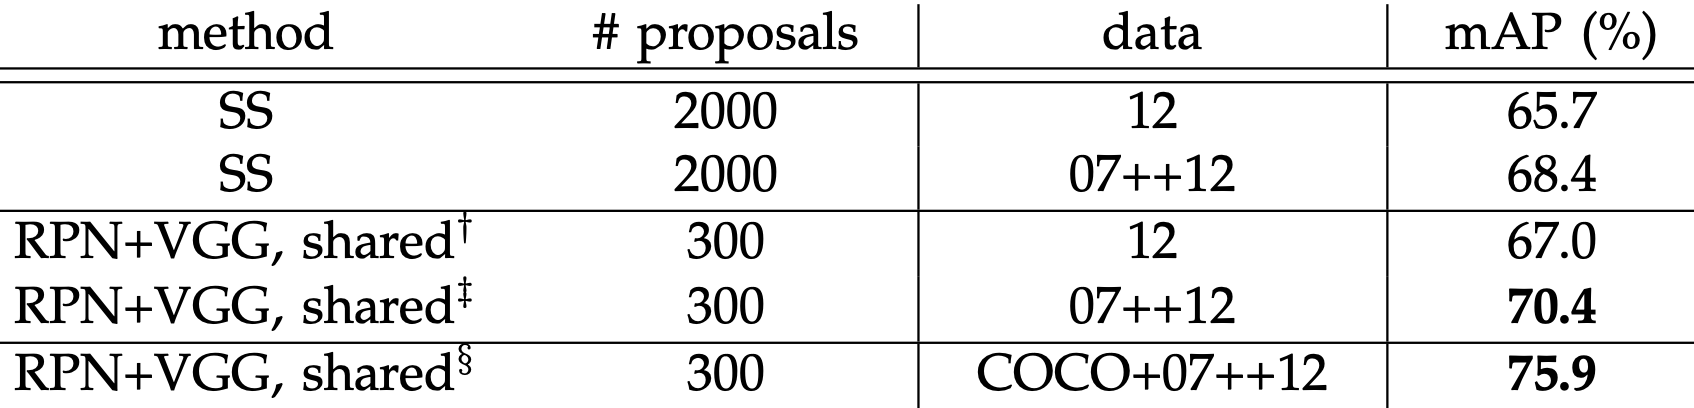
\includegraphics[width=10cm] {images/faster_rcnn_results_3}
    %     \caption{Kết quả của mô hình Fast R-CNN sử dụng RPN và backbone VGG-16 so sánh với mô hình Fast R-CNN sử dụng thuật toán Selective Search trên bộ dữ liệu VOC 2012 test với các bộ dữ liệu huấn luyện khác nhau. (Nguồn: \cite{ren2015faster})}
    %     \label{fig:faster_rcnn_results_3}
    % \end{figure}

    % \noindent
    % Cuối cùng, so sánh về mặt tốc độ, nhóm tác giả so sánh kết quả của các mô hình Faster R-CNN (dùng backbone là VGG-16, ký hiệu là \textbf{VGG, RPN + Fast R-CNN}), mô hình Faster R-CNN (dùng backbone là ZF-Net, ký hiệu là \textbf{ZF, RPN + Fast R-CNN}) với mô hình Fast R-CNN sử dụng thuật toán Selective Search (dùng backbone là VGG-16, ký hiệu là \textbf{VGG, SS + Fast R-CNN}).
    % Trong đó, thời gian (tính theo đơn vị ms) xử lý lớp conv được thống kê tại cột \textbf{conv}, thời gian đề xuất các khu vực được thống kê tại cột \textbf{proposals}, thời gian xử lý các bước như NMS, lớp pooling, lớp fully connected \index{lớp fully connected} và lớp softmax được thống kê tại cột \textbf{region-wise}, tổng thời gian xử lý toàn bộ được thống kê tại cột \textbf{total}, số lượng ảnh xử lý trong một giây được thống kê tại cột \textbf{rate}. \\
    % Kết quả, mô hình \textbf{VGG, RPN + Fast R-CNN} nhanh hơn \textbf{VGG, SS + Fast R-CNN} gần 10 lần, trong đó, thời gian đề xuất khu vực được tiết kiệm tới 150 lần.
    % Mô hình \textbf{ZF, RPN + Fast R-CNN} thậm chí còn nhanh gấp gần bốn lần mô hình \textbf{VGG, RPN + Fast R-CNN}, đạt số khung hình trên một giây là 17 fps.

    % \begin{figure}[H]
    %     \centering
    %     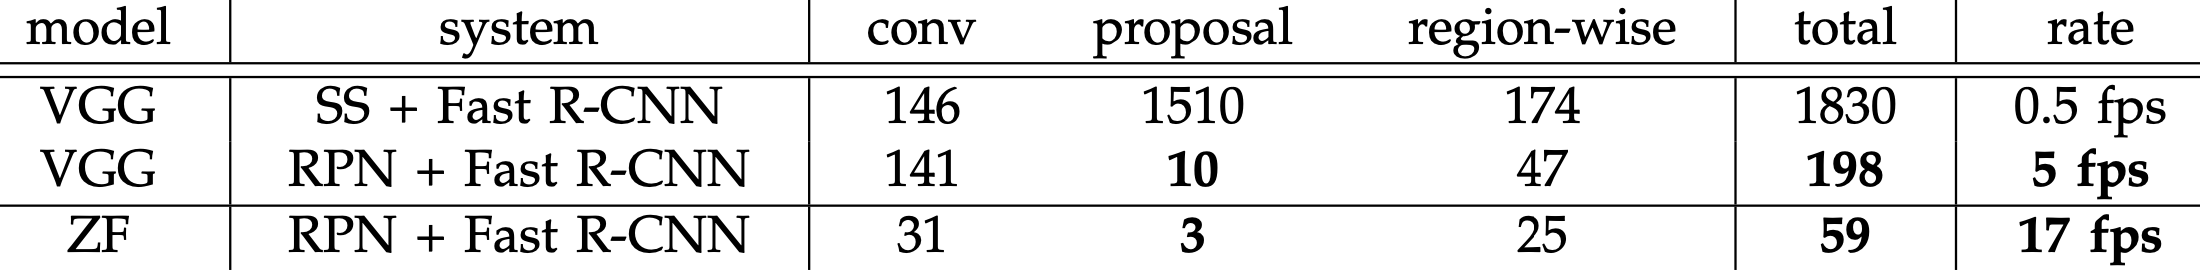
\includegraphics[width=10cm] {images/faster_rcnn_results_4}
    %     \caption{Toàn cảnh sự kết hợp của mô hình Region Proposal Network và Fast R-CNN tạo ra mô hình Faster R-CNN (Nguồn: \cite{ren2015faster})}
    %     \label{fig:faster_rcnn_results_4}
    % \end{figure}

    \noindent
    \textbf{\textit{Vấn đề tồn đọng của mô hình Faster R-CNN}} \\
    Kết quả của mô hình Faster R-CNN và tâm điểm là kiến trúc RPN giúp thay thế thuật toán Selective Search đã giúp cho Faster R-CNN đạt độ chính xác cao hơn so với mô hình Fast R-CNN sử dụng Selective Search.
    Hơn nữa, RPN giúp cho Faster R-CNN nhanh hơn tới 10 lần so với cấu hình tương tự Fast R-CNN sử dụng Selective Search.
    Điều này giúp cho Faster R-CNN cho đến nay vẫn là một mô hình tốt để giải quyết bài toán object detection, vừa đạt độ chính xác cao, vừa có tốc độ tương đối tốt.
    Tuy nhiên, cho đến thời điểm thực hiện luận văn này, đã có nhiều mô hình khác hiện đại hơn chỉ ra những vấn đề tồn đọng của Faster R-CNN như độ chính xác cần phải cải thiện thêm hay tốc độ chưa đạt đến ngưỡng chạy trong thời gian thực. 
}
    \fasterrcnn

    \subsection{Kiến trúc Feature Pyramid Networks}
    \def\fpn{
    Các kiến trúc backbone \index{backbone} như AlexNet \index{AlexNet} \cite{krizhevsky2012imagenet}, VGG \index{VGG} \cite{simonyan2014very}, InceptionNet \index{InceptionNet} \cite{szegedy2015going}, SqueezeNet \index{SqueezeNet} \cite{iandola2016squeezenet} và đặc biệt là ResNet \index{ResNet} \cite{he2016deep} đã đạt những thành công nhất định.
    Tuy nhiên, các kiến trúc backbone \index{backbone} trên vẫn gặp phải một vấn đề về chênh lệch kích thước giữa các đối tượng trong ảnh.
    Feature Pyramid Networks \index{Feature Pyramid Networks} \cite{lin2017feature} (gọi tắt là FPN \index{FPN}) được giới thiệu như một kiến trúc backbone \index{backbone} nhằm giải quyết vấn đề trên.
    Việc sử dụng FPN \index{FPN} như là kiến trúc backbone \index{backbone} kết hợp cùng mô hình Faster R-CNN \index{Faster R-CNN} \index{Faster R-CNN} \cite{ren2015faster} đã vượt qua rất nhiều các mô hình nhận diện đối tượng \index{nhận diện đối tượng} khác để trở thành mô hình tốt nhất ở thời điểm đó.

    \noindent
    \textbf{\textit{So sánh các kiến trúc pyramid \index{kiến trúc pyramid} khác nhau}}

    \begin{figure}[H]
        \centering
        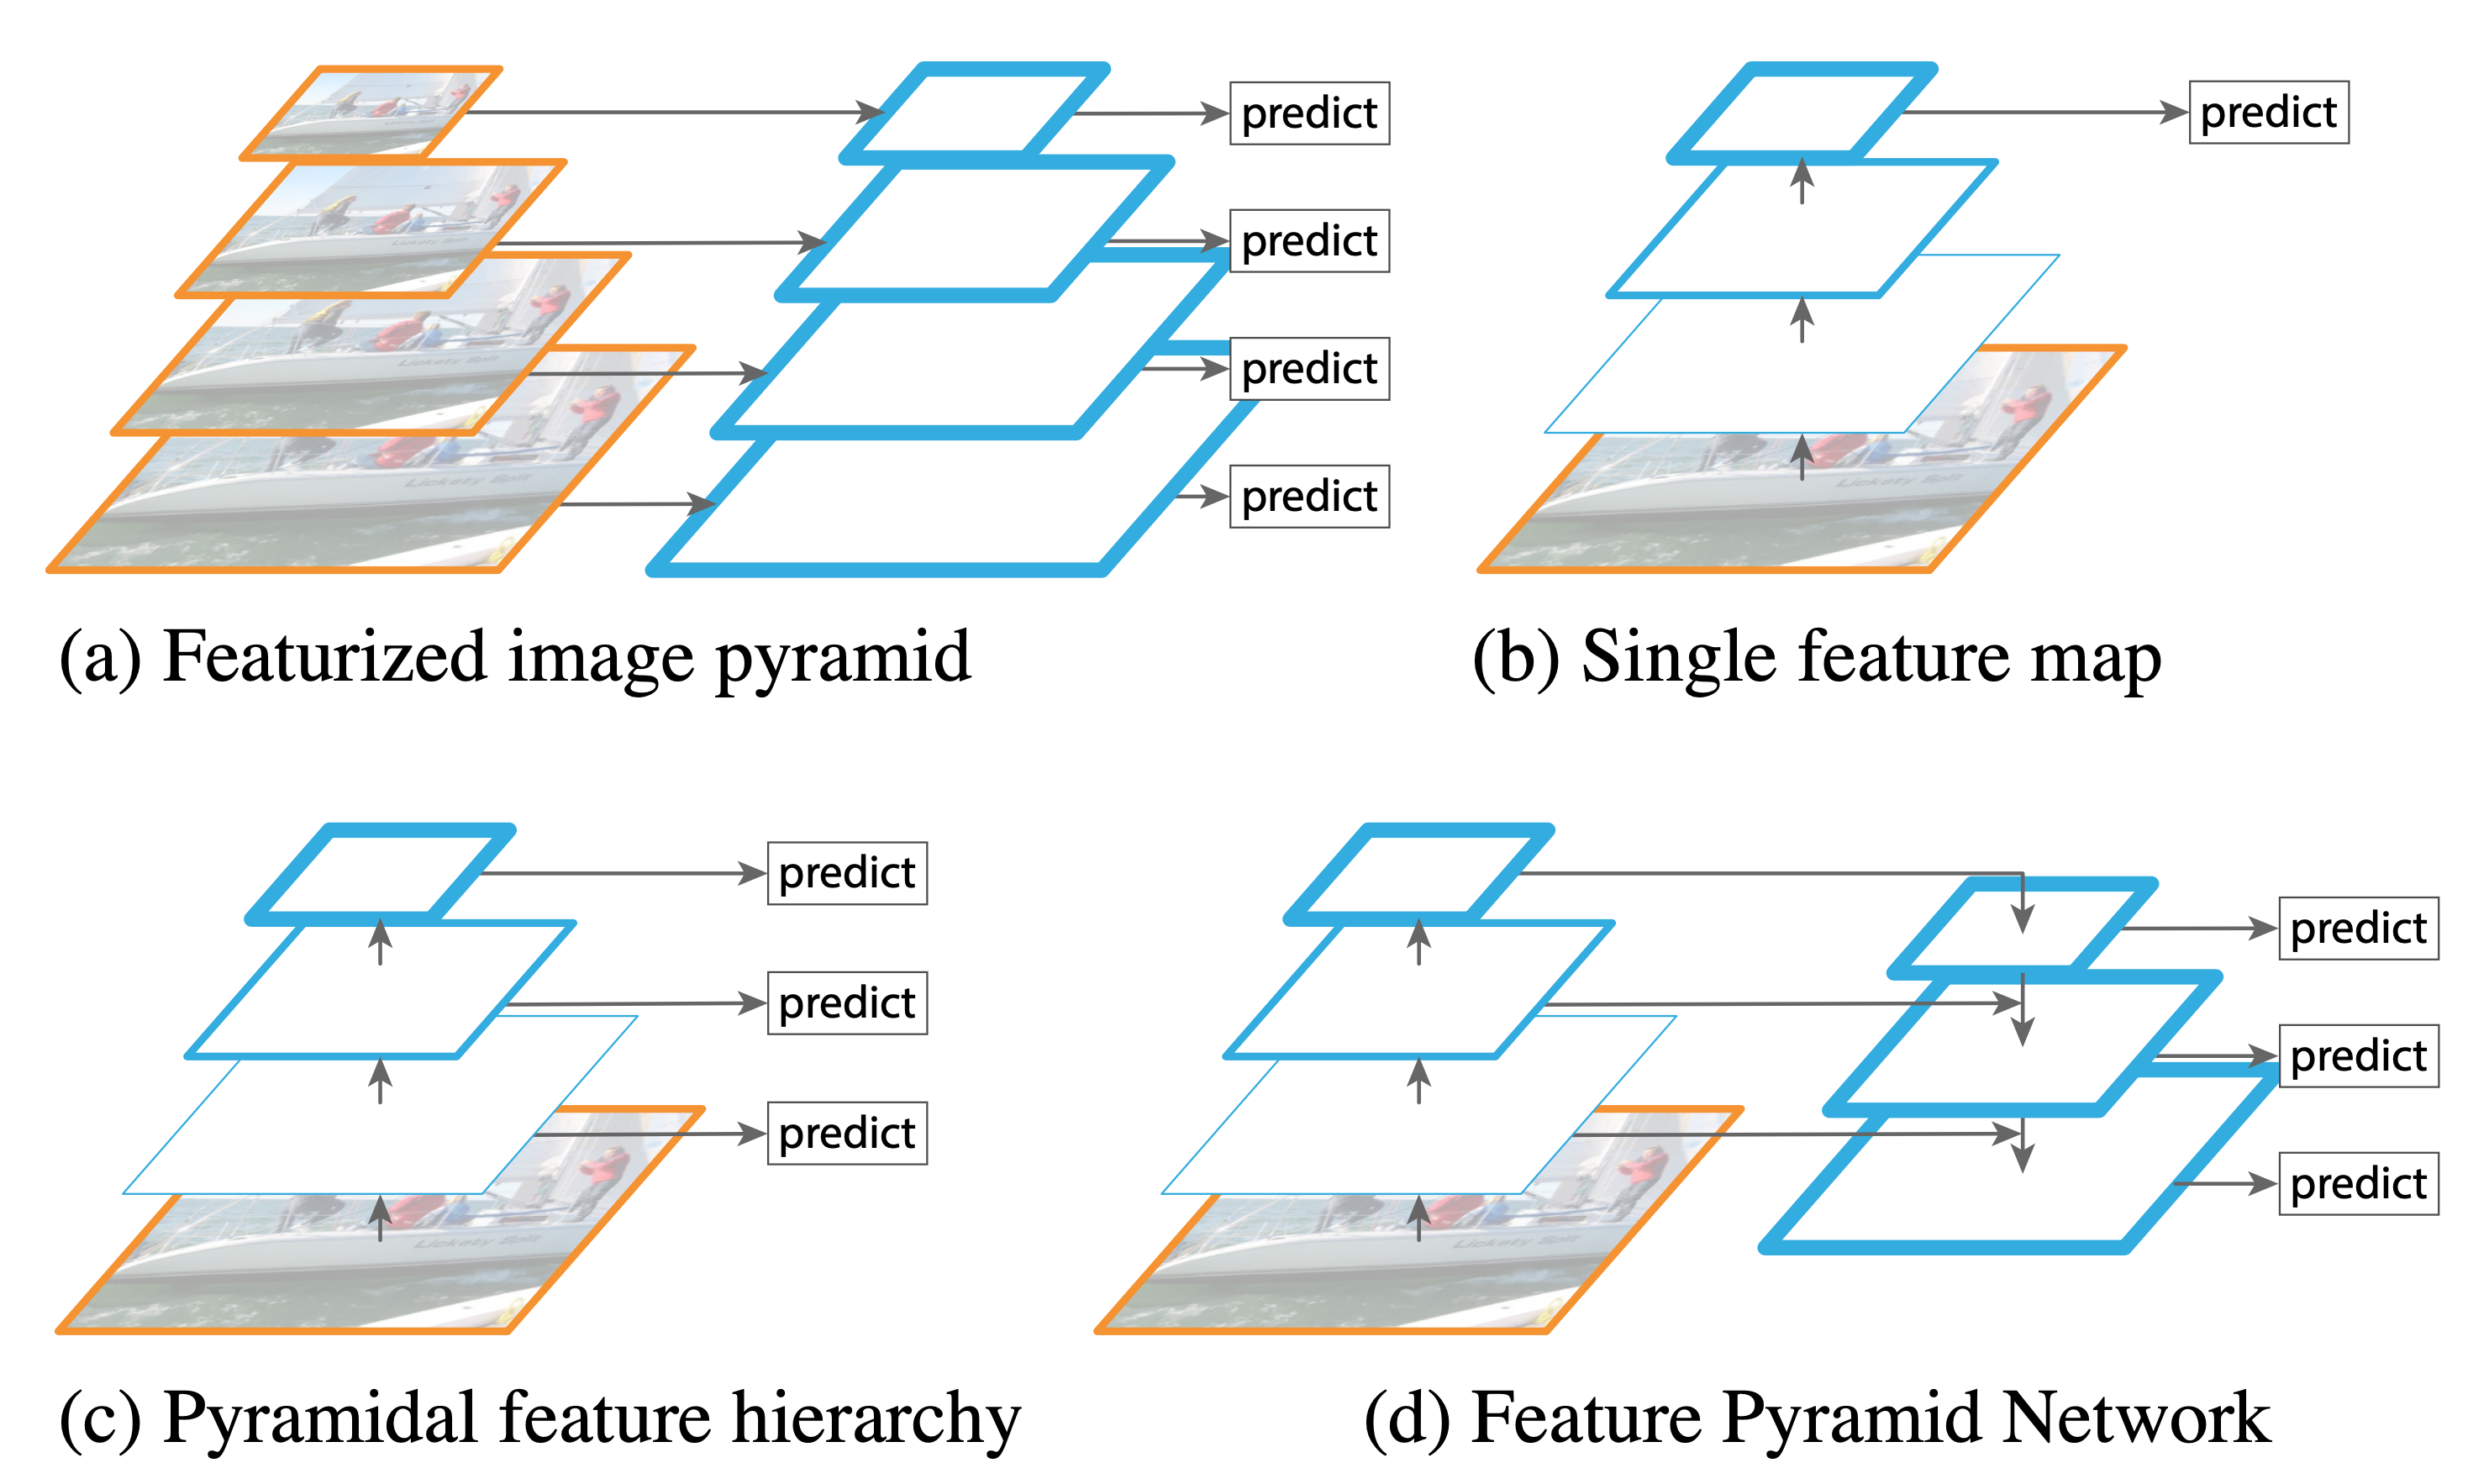
\includegraphics[width=11cm] {images/fpn_compare}
        \caption{So sánh các kiến trúc pyramid \index{kiến trúc pyramid} khác nhau (Nguồn: \cite{lin2017feature})}
        \label{fig:fpn_compare}
    \end{figure}

    \noindent
    Ý tưởng về việc xây dựng và sử dụng các đặc trưng của ảnh với nhiều kích thước khác nhau không mới, tuy nhiên, các giải pháp đã có vào thời điểm đó đều vướng phải một số vấn đề: \\
    - \textit{Featurized image pyramid} \index{Featurized image pyramid}: Việc sử dụng nhiều kích thước ảnh khác nhau để tạo ra nhiều đặc trưng có kích thước khác nhau một cách độc lập là ý tưởng cơ bản nhất. Mặc dù đạt được hiệu quả cao về độ chính xác khi khai thác ảnh đầu vào với nhiều kích thước khác nhau, nhưng phương pháp này khiến cho mô hình giải bài toán nhận diện đối tượng \index{nhận diện đối tượng} trở nên cồng kềnh và tốn rất nhiều thời gian để xử lý và gần như bất khả thi để có thể huấn luyện được mô hình. \\
    - \textit{Single feature map} \index{Single feature map}: Việc sử dụng chỉ một kích thước đặc trưng duy nhất giúp cho mô hình xử lý nhanh hơn nhưng lại khiến cho mô hình khó có thể học được những đặc trưng giữa các đối tượng có kích thước chênh lệch trong ảnh. Đặc biệt, việc đưa ảnh đầu vào qua nhiều khối Conv đã loại bỏ rất nhiều thông tin và gần như không còn thông tin để mô hình có thể nhận biết được các đối tượng có kích thước nhỏ. \\
    - \textit{Pyramidal feature hierarchy} \index{Pyramidal feature hierarchy}: Việc sử dụng nhiều feature maps \index{feature maps} có kích thước khác nhau cùng đưa ra kết quả được sử dụng trong mô hình nhận diện đối tượng \index{nhận diện đối tượng} khá nổi tiếng là SSD \index{SSD} \cite{liu2016ssd}. Tuy nhiên, thay vì tận dụng toàn bộ các feature maps \index{feature maps} sinh ra từ các khối Conv của backbone \index{backbone} VGG-16 \index{VGG-16}, SSD \index{SSD} chỉ sử dụng feature maps \index{feature maps} từ khối Conv thứ 5 và bổ sung thêm các lớp Conv \index{lớp Conv}. Điều này khiến cho SSD \index{SSD} bỏ qua những feature maps \index{feature maps} có kích thước lớn, có ý nghĩa quan trọng trong việc detect các đối tượng có kích thước nhỏ. \\
    - \textit{Feature Pyramid Network} \index{Feature Pyramid Network}: Dựa trên vấn đề trên từ SSD \index{SSD}, nhóm tác giả đề xuất FPN \index{FPN} tận dụng tối đa các feature maps \index{feature maps} trích xuất được từ backbone \index{backbone} nhằm tạo ra bộ feature maps \index{feature maps} mới gồm nhiều kích thước khác nhau và chứa rất nhiều thông tin về nội dung của ảnh đầu vào. Để đạt được điều này, nhóm tác giả thiết kế kiến trúc kết hợp những feature maps \index{feature maps} có kích thước lớn và những feature maps \index{feature maps} có kích thước nhỏ bằng top-down pathway \index{top-down pathway} và lateral connections \index{lateral connections}.

    \noindent
    \textbf{\textit{Kiến trúc mô hình Feature Pyramid Networks}} \\
    Ý tưởng về việc sử dụng kiến trúc mô hình theo dạng top-down không phải là mới và đã được nhắc đến trong một số nghiên cứu. Tuy nhiên, điểm giống nhau của các nghiên cứu có thiết kế mô hình theo kiểu top-down đó là mô hình chỉ sử dụng một feature maps \index{feature maps} cuối cùng, sau khi đã tổng hợp các thông tin trong suốt quá trình top-down, để đưa ra quyết định dự đoán cuối cùng.

    \noindent
    Trong khi đó, đối với FPN, nhóm tác giả đưa ra quyết định dự đoán trên từng feature maps \index{feature maps} trong suốt quá trình top-down. Từ đó, đặc biệt nâng cao chất lượng của mô hình nhận diện đối tượng \index{nhận diện đối tượng} khi có thể vừa trích xuất được thông tin của các đối tượng có kích thước lớn từ các feature maps \index{feature maps} có kích thước nhỏ vừa trích xuất được thông tin của các đối tượng có kích thước nhỏ từ các feature maps \index{feature maps} có kích thước lớn.

    \begin{figure}[H]
        \centering
        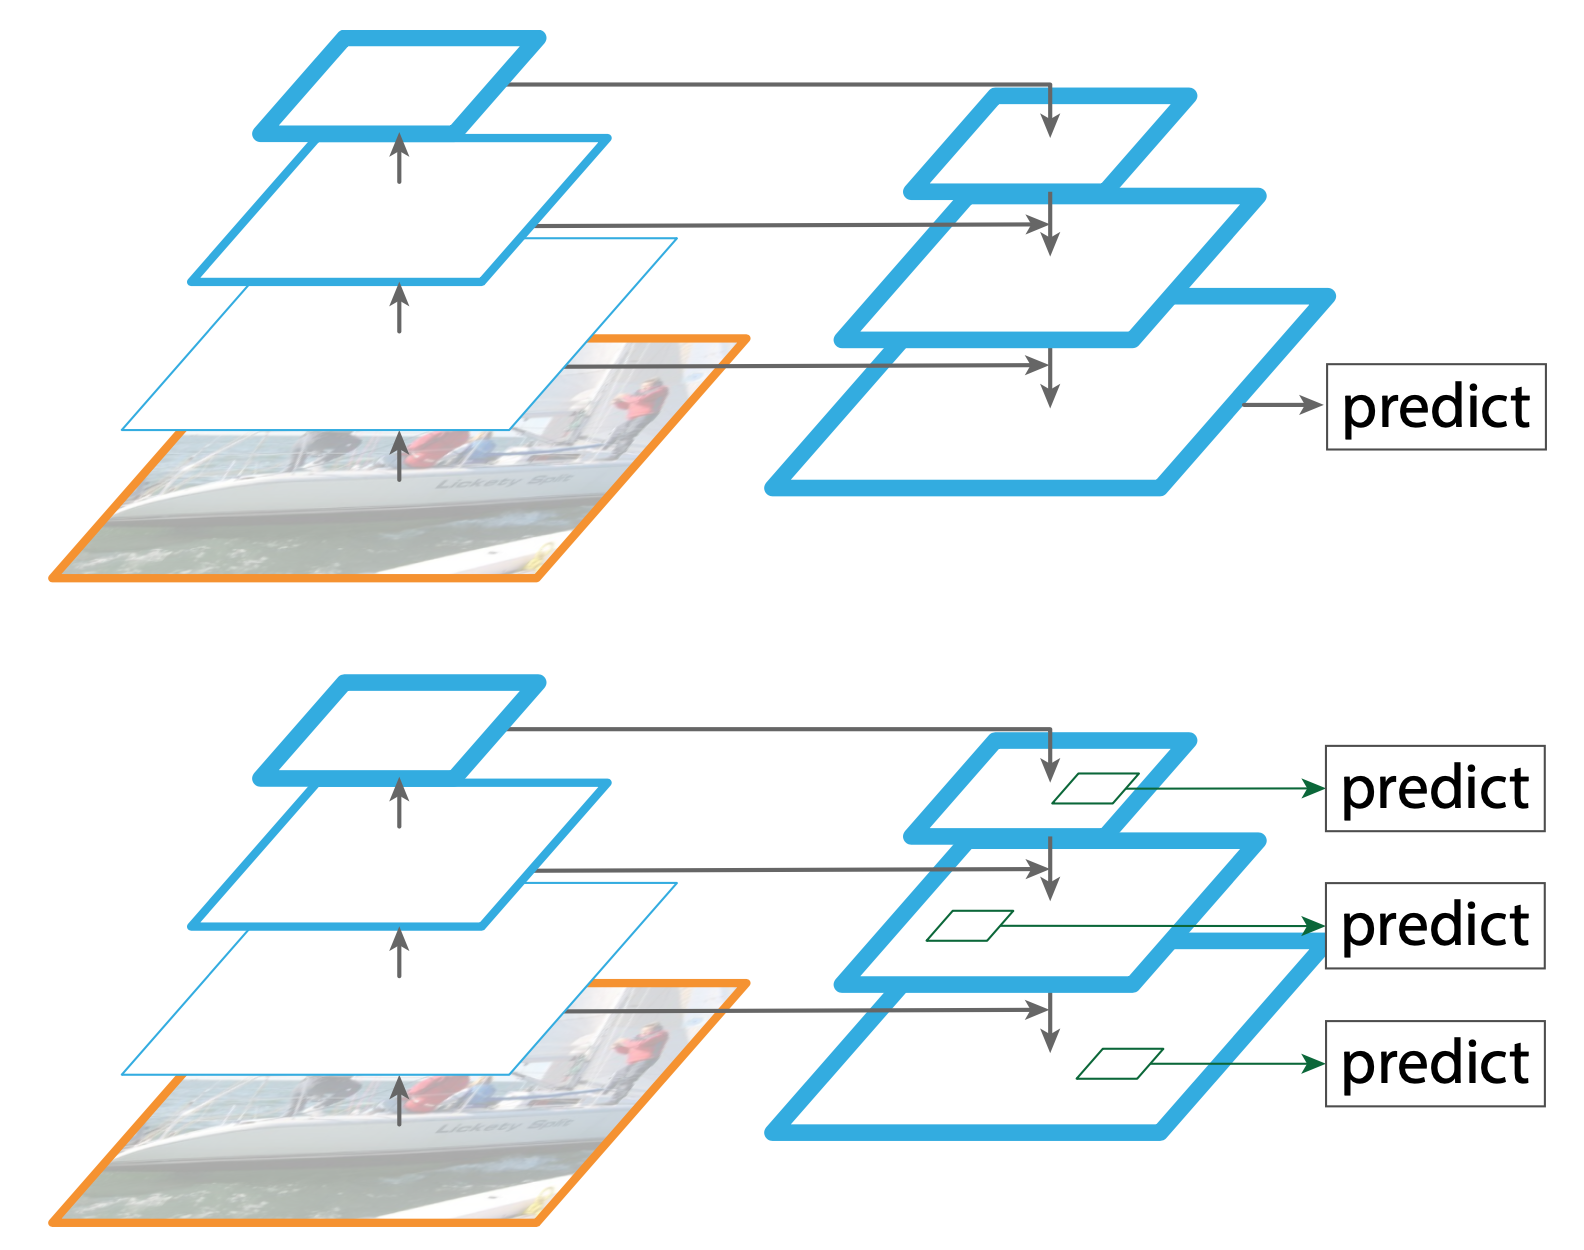
\includegraphics[width=6cm] {images/fpn_topdown}
        \caption{So sánh các kiến trúc theo dạng top-down khác nhau (Nguồn: \cite{lin2017feature})}
        \label{fig:fpn_topdown}
    \end{figure}

    \noindent
    Kiến trúc FPN \index{FPN} có thể được áp dụng với nhiều backbone \index{backbone} Conv khác nhau như AlexNet, VGG hay ResNet, cụ thể trong nghiên cứu, nhóm tác giả lựa chọn ResNet làm mô hình backbone.
    Kiến trúc FPN \index{FPN} có thể được chia làm hai phần: \\
    - \textit{Bottom-up pathway} \index{bottom-up pathway} là quá trình mà ta đưa ảnh đầu vào qua mô hình backbone \index{backbone} Conv như ResNet và thu được các feature maps \index{feature maps}.
    Tuy nhiên, trong các mô hình backbone \index{backbone} Conv, sẽ có một nhóm các lớp Conv \index{lớp Conv} tạo ra các feature maps \index{feature maps} có kích thước giống nhau, và nhóm các lớp Conv \index{lớp Conv} này được gọi là một khối Conv.
    Đối với FPN, nhóm tác giả lựa chọn các feature maps \index{feature maps} được sinh ra từ các lớp Conv \index{lớp Conv} cuối cùng trong mỗi khối Conv để sử dụng cho nhánh top-down pathway \index{top-down pathway}.
    Cụ thể đối với mô hình backbone \index{backbone} ResNet, nhóm tác giả sử dụng các feature maps \index{feature maps} được sinh ra từ residual block cuối cùng của mỗi khối Conv (trừ khối Conv đầu tiên do kích thước của feature maps \index{feature maps} này lớn và gây ra vấn đề về bộ nhớ), ký hiệu là \textit{{${C}_{2}, {C}_{3}, {C}_{4}, {C}_{5}$}}.
    Các feature maps \index{feature maps} này có kích thước lần lượt bằng 1/4, 1/8, 1/16 và 1/32 so với kích thước của ảnh đầu vào. \\
    - \textit{Top-down pathway và lateral connections} \index{top-down pathway} \index{lateral connections} là quá trình mà FPN \index{FPN} sinh ra thêm các feature maps \index{feature maps} mới từ các feature maps \index{feature maps} của bottom-up pathway \index{bottom-up pathway} và kết hợp chúng lại thông qua lateral connections \index{lateral connections}.
    Cụ thể, các feature maps \index{feature maps} của bottom-up pathway \index{bottom-up pathway} được đưa qua các lớp Conv \index{lớp Conv} có kích thước 1x1, stride \index{stride} bằng 1 nhằm giữ nguyên kích thước chiều dài, chiều rộng và chỉ thay đổi kích thước chiều channel \index{channel} của feature maps \index{feature maps}.
    Các feature maps \index{feature maps} ở vị trí cao hơn (có kích thước nhỏ hơn) được upsample \index{upsample} thông qua thuật toán nearest neighbor \index{nearest neighbor} và cộng ma trận với feature maps \index{feature maps} đầu ra từ lớp Conv \index{lớp Conv} 1x1 nói trên.
    Cuối cùng, các feature maps \index{feature maps} đầu ra từ phép cộng ma trận nói trên được đi qua một lớp Conv \index{lớp Conv} 3x3 có cùng số đầu ra channel \index{channel} của feature maps \index{feature maps} nhằm giảm bớt hiệu ứng của thuật toán nearest neighbor \index{nearest neighbor} và tạo ra các feature maps \index{feature maps} đầu ra cuối cùng có cùng số channel \index{channel} với nhau.
    Tập hợp feature maps \index{feature maps} này được gọi là \textit{{${P}_{2}, {P}_{3}, {P}_{4}, {P}_{5}$}} tương ứng với các feature maps \index{feature maps} có cùng kích thước \textit{{${C}_{2}, {C}_{3}, {C}_{4}, {C}_{5}$}}.

    \begin{figure}[H]
        \centering
        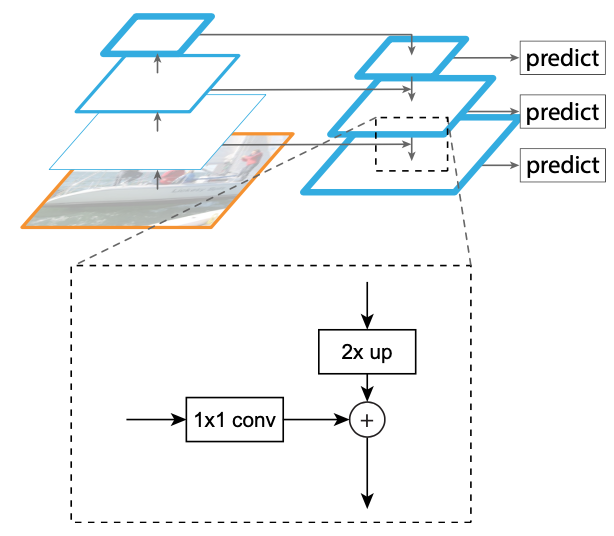
\includegraphics[width=6cm] {images/fpn_detail}
        \caption{Chi tiết kiến trúc FPN (Nguồn: \cite{lin2017feature})}
        \label{fig:fpn_detail}
    \end{figure}

    % \noindent
    % \textbf{\textit{Sử dụng kiến trúc FPN cho mô hình RPN}} \\
    % Ý tưởng về việc sử dụng kiến trúc FPN \index{FPN} cho mô hình RPN \index{RPN} \cite{ren2015faster} được nhóm tác giả đề xuất nhằm cải thiện khả năng đề xuất ra các khu vực có kích thước chênh lệch nhau.
    % Cụ thể, thay vì việc sử dụng một feature maps \index{feature maps} thu được từ feature extraction module \index{feature extraction module}, nhóm tác giả sử dụng các feature maps \index{feature maps} \textit{{${P}_{2}, {P}_{3}, {P}_{4}, {P}_{5}, {P}_{6}$}} (nhóm tác giả sử dụng thêm feature maps \index{feature maps} ${P}_{6}$ nhằm đề xuất ra những khu vực có kích thước lớn hơn).
    % Các feature maps \index{feature maps} này cùng được đưa qua một bộ các lớp Conv \index{lớp Conv} 3x3 và 1x1 chung để trả đầu ra kết quả anchor \index{anchor} có chứa đối tượng hay không và toạ độ của khu vực mà mô hình đề xuất.
    % Với việc sử dụng nhiều feature maps \index{feature maps} có các kích thước khác nhau, trên mỗi feature maps \index{feature maps}, nhóm tác giả chỉ sử dụng một kích thước anchor \index{anchor} lần lượt tương ứng \textit{{${32}^{2}, {64}^{2}, {128}^{2}, {256}^{2}, {512}^{2},$}} với ba tỷ lệ chiều dài giữa chiều rộng là \textit{1:2, 1:1, 2:1}.
    % Để có thể huấn luyện được, nhóm tác giả cũng sử dụng cơ chế gán positive/negative anchor \index{anchor} tương tự như chiến lược được đề xuất trong \cite{ren2015faster}.

    % \begin{figure}[H]
    %     \centering
    %     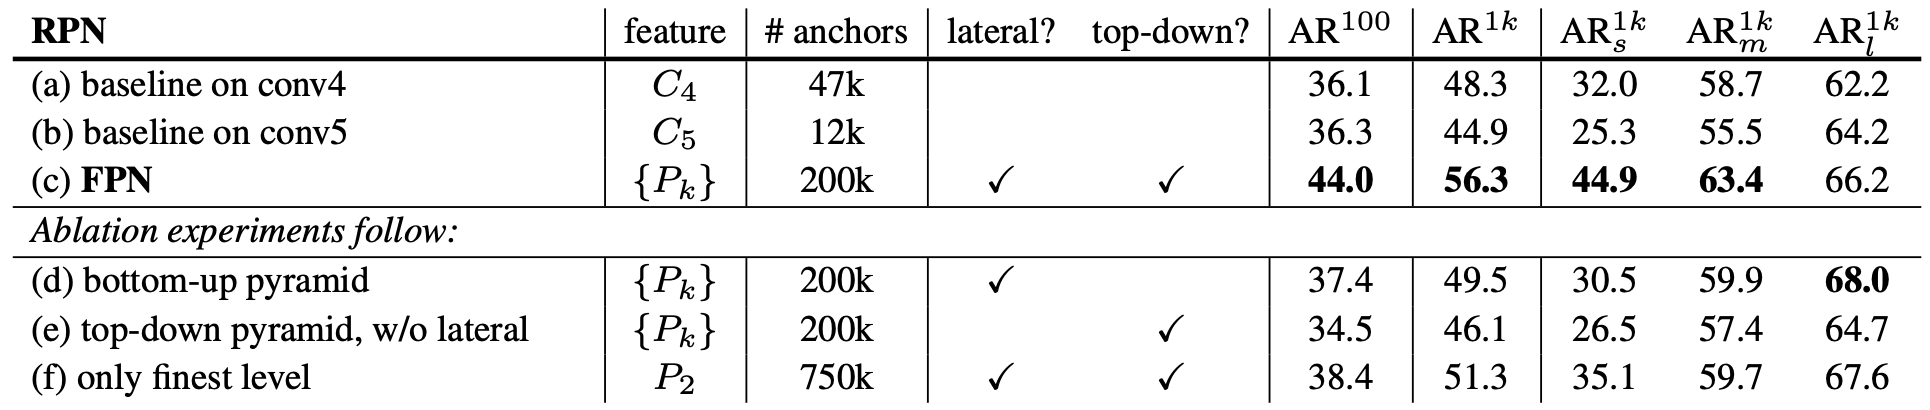
\includegraphics[width=12cm] {images/fpn_results_1}
    %     \caption{Kết quả của thí nghiệm sử dụng kiến trúc FPN cho mô hình RPN \index{RPN} \cite{ren2015faster} (Nguồn: \cite{lin2017feature})}
    %     \label{fig:fpn_results}
    % \end{figure}

    % \noindent
    % Kết quả của thí nghiệm sử dụng kiến trúc FPN \index{FPN} cho mô hình RPN \index{RPN} \cite{ren2015faster} được nhóm tác giả chia sẻ khá khả quan.
    % Ngoài việc so sánh việc sử dụng kiến trúc FPN \index{FPN} với các kiến trúc trước đây của mô hình RPN, nhóm tác giả còn so sánh thêm một số cấu hình khác của kiến trúc FPN \index{FPN}.
    % Cụ thể các cấu hình như sau: \\
    % - \textit{baseline on conv4} là cấu hình sử dụng feature maps \index{feature maps} từ lớp Conv \index{lớp Conv} thứ 4 của feature extraction module \index{feature extraction module} cho mô hình RPN. \\
    % - \textit{baseline on conv5} là cấu hình sử dụng feature maps \index{feature maps} từ lớp Conv \index{lớp Conv} thứ 5 của feature extraction module \index{feature extraction module} cho mô hình RPN. \\
    % - \textit{FPN} là cấu hình sử dụng kiến trúc FPN trích xuất các feature maps \index{feature maps} cho mô hình RPN. \\
    % - \textit{bottom-up pyramid} là cấu hình sử dụng các feature maps \index{feature maps} \textit{{${P}_{2}, {P}_{3}, {P}_{4}, {P}_{5}, {P}_{6}$}} cho mô hình RPN.
    % Tuy nhiên, giữa các feature maps \index{feature maps} này không có top-down pathway với nhau (hay nói cách khác, các feature maps \index{feature maps} \textit{{${P}_{2}, {P}_{3}, {P}_{4}, {P}_{5}, {P}_{6}$}} được sinh một cách độc lập từ các feature maps \index{feature maps} \textit{{${C}_{2}, {C}_{3}, {C}_{4}, {C}_{5}, {C}_{6}$}}). \\
    % - \textit{top-down pyramid, w/o lateral} là cấu hình sử dụng các feature maps \index{feature maps} \textit{{${P}_{2}, {P}_{3}, {P}_{4}, {P}_{5}, {P}_{6}$}} cho mô hình RPN.
    % Tuy nhiên, giữa các feature maps \index{feature maps} \textit{{${P}_{3}, {P}_{4}, {P}_{5}, {P}_{6}$}} không có lateral connections \index{lateral connections} với các feature maps \index{feature maps} \textit{{${C}_{3}, {C}_{4}, {C}_{5}, {C}_{6}$}} (hay nói cách khác, các feature maps \index{feature maps} \textit{{${P}_{3}, {P}_{4}, {P}_{5}, {P}_{6}$}} chỉ được sinh từ các feature maps \index{feature maps} \textit{{${P}_{2}, {P}_{3}, {P}_{4}, {P}_{5}$}}). \\
    % - \textit{only finest level} là cấu hình chỉ sử dụng duy nhất feature maps \index{feature maps} \textit{${P}_{2}$} cho mô hình RPN. \\
    % Trong đó, tất cả các cấu hình được huấn luyện với bộ dữ liệu \textit{COCO trainval135k} và kết quả thu được đánh giá trên bộ dữ liệu \textit{COCO minival}.
    % feature maps \index{feature maps} sử dụng trong cấu hình được ghi chú tại cột \textbf{feature}, số lượng khu vực được đề xuất trong quá trình test được thống kê tại cột \textbf{\# anchors}, cấu hình có sử dụng lateral connections \index{lateral connections} và top-down pathway hay không được chú thích tại cột \textbf{lateral} và \textbf{top-down}. \\
    % Cấu hình \textit{FPN} đạt kết quả cao hơn vượt trội so với các cấu hình \textit{baseline on conv4} và \textit{baseline on conv5} nguyên bản.
    % Cấu hình \textit{FPN} chỉ đạt kết quả kém hơn so với cấu hình \textit{bottom-up pyramid} khi so sánh trên chỉ số đánh giá với những bounding box \index{bounding box} có kích thước lớn, tuy nhiên, sự chênh lệch giữa hai cấu hình là không quá khác biệt.

    % \noindent
    % \textbf{\textit{Sử dụng kiến trúc FPN cho mô hình Fast R-CNN \index{Fast R-CNN}}} \\
    % Ý tưởng về việc sử dụng kiến trúc FPN cho mô hình Fast R-CNN \index{Fast R-CNN} được nhóm tác giả đề xuất nhằm cải thiện khả năng định vị ra bounding box \index{bounding box} từ các khu vực đã được đề xuất từ mô hình RPN.
    % Cụ thể, sau khi đưa ảnh qua region proposals module \index{region proposals module} của mô hình Fast R-CNN \index{Fast R-CNN} là Selective Search, ta thu được toạ độ của khu vực được đề xuất trên ảnh đầu vào.
    % Đối với mô hình Fast R-CNN \index{Fast R-CNN} nguyên bản, ta dễ dàng lấy được khu vực đề xuất trên feature maps \index{feature maps} của ảnh đầu vào, tuy nhiên, với việc sử dụng kiến trúc FPN cho feature extraction module \index{feature extraction module}, câu hỏi đặt ra là đối với từng khu vực đề xuất ta xác định feature maps \index{feature maps} nào trong số \textit{{${P}_{2}, {P}_{3}, {P}_{4}, {P}_{5}$}} để lấy làm đầu vào cho lớp RoI pooling?
    % Nhóm tác giả đã coi danh sách feature maps \index{feature maps} \textit{{${P}_{2}, {P}_{3}, {P}_{4}, {P}_{5}$}} sinh ra bởi FPN tương tự với các feature maps \index{feature maps} được sinh ra từ việc sử dụng image pyramids và áp dụng công thức sau để xác định feature maps \index{feature maps} phù hợp cho từng khu vực làm đầu vào của lớp RoI pooling.

    % \begin{equation}
    %     \label{eq:roi_mapping}
    %     k = \lfloor k_0 + \log_2(\sqrt{wh} / 224) \rfloor.
    % \end{equation}

    % \noindent
    % trong đó: \\
    % \textit{k} là index của feature maps \index{feature maps} sử dụng làm đầu vào cho lớp RoI pooling tương ứng với khu vực đề xuất có kích thước chiều rộng là \textit{w} và chiều cao là \textit{h} \\
    % $k_0$ là index của feature maps \index{feature maps} sử dụng làm đầu vào cho lớp RoI pooling tương ứng với khu vực đề xuất có kích thước chiều rộng và chiều cao lần lượt là 224 và 224 \\
    % Tác giả lựa chọn con số 224 bởi đây là kích thước ảnh của pretrained ImageNet và lựa chọn $k_0 = 4$. \\
    % Các feature maps \index{feature maps} được lấy ra tương ứng với từng khu vực đề xuất được đưa qua lớp lớp RoI pooling có kích thước đầu ra là 7x7 và được đưa qua chung các lớp Conv \index{lớp Conv} và lớp fully connected \index{lớp fully connected} để xác định lớp của đối tượng và toạ độ của bounding box \index{bounding box}.

    % \begin{figure}[H]
    %     \centering
    %     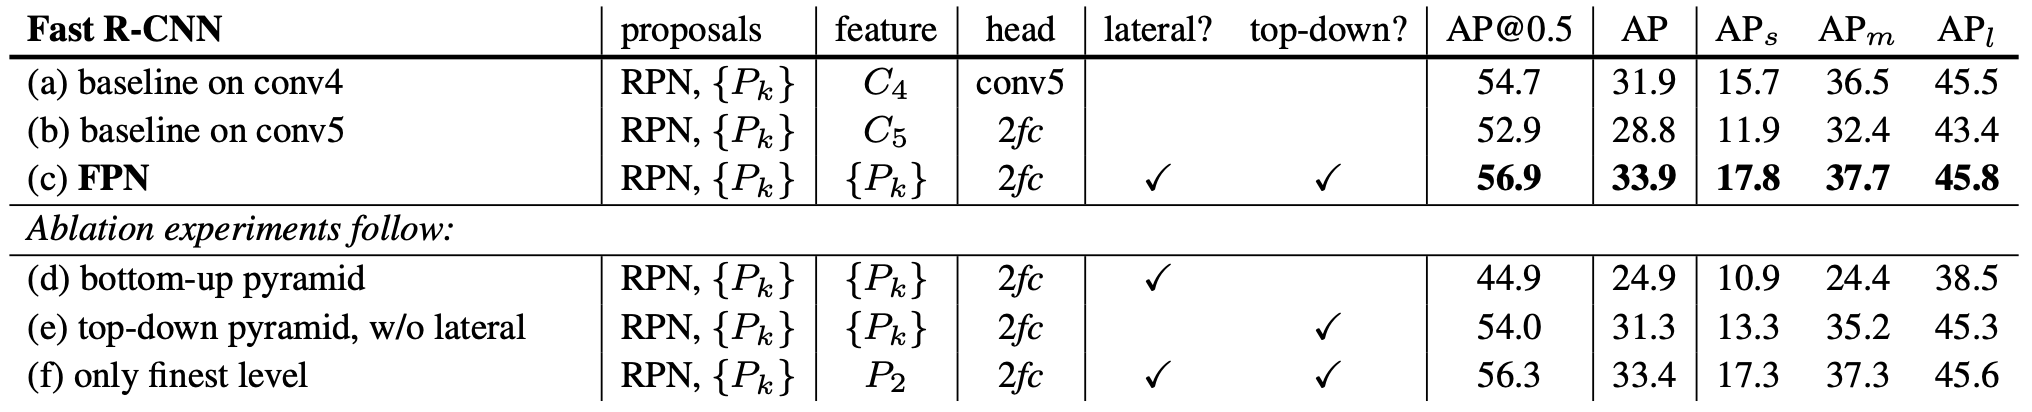
\includegraphics[width=12cm] {images/fpn_results_2}
    %     \caption{Kết quả của thí nghiệm sử dụng kiến trúc FPN cho mô hình Fast R-CNN \index{Fast R-CNN} (Nguồn: \cite{lin2017feature})}
    %     \label{fig:fpn_results}
    % \end{figure}
    
    % \noindent
    % Kết quả của thí nghiệm sử dụng kiến trúc FPN cho mô hình Fast R-CNN \index{Fast R-CNN} được nhóm tác giả chia sẻ khá ấn tượng.
    % Ngoài việc so sánh việc sử dụng kiến trúc FPN với các kiến trúc trước đây của mô hình Fast R-CNN \index{Fast R-CNN}, nhóm tác giả còn so sánh thêm một số cấu hình khác của kiến trúc FPN.
    % Cụ thể các cấu hình như sau: \\
    % - \textit{baseline on conv4} là cấu hình sử dụng feature maps \index{feature maps} từ lớp Conv \index{lớp Conv} thứ 4 của feature extraction module \index{feature extraction module} cho mô hình Fast R-CNN \index{Fast R-CNN}. \\
    % - \textit{baseline on conv5} là cấu hình sử dụng feature maps \index{feature maps} từ lớp Conv \index{lớp Conv} thứ 5 của feature extraction module \index{feature extraction module} cho mô hình Fast R-CNN \index{Fast R-CNN}. \\
    % - \textit{FPN} là cấu hình sử dụng kiến trúc FPN trích xuất feature maps \index{feature maps} cho mô hình Fast R-CNN \index{Fast R-CNN} như mô tả ở trên. \\
    % - \textit{bottom-up pyramid} là cấu hình sử dụng các feature maps \index{feature maps} \textit{{${P}_{2}, {P}_{3}, {P}_{4}, {P}_{5}, {P}_{6}$}} cho mô hình Fast R-CNN \index{Fast R-CNN}.
    % Tuy nhiên, giữa các feature maps \index{feature maps} này không có top-down pathway với nhau (hay nói cách khác, các feature maps \index{feature maps} \textit{{${P}_{2}, {P}_{3}, {P}_{4}, {P}_{5}, {P}_{6}$}} được sinh một cách độc lập từ các feature maps \index{feature maps} \textit{{${C}_{2}, {C}_{3}, {C}_{4}, {C}_{5}, {C}_{6}$}}). \\
    % - \textit{top-down pyramid, w/o lateral} là cấu hình sử dụng các feature maps \index{feature maps} \textit{{${P}_{2}, {P}_{3}, {P}_{4}, {P}_{5}, {P}_{6}$}} cho mô hình Fast R-CNN \index{Fast R-CNN}.
    % - \textit{only finest level} là cấu hình chỉ sử dụng duy nhất feature maps \index{feature maps} \textit{${P}_{2}$} cho mô hình Fast R-CNN \index{Fast R-CNN}. \\
    % Trong đó, tất cả các cấu hình được huấn luyện với bộ dữ liệu \textit{COCO trainval135k} và kết quả thu được đánh giá trên bộ dữ liệu \textit{COCO minival} và cùng sử dụng chung một bộ khu vực đề xuất từ mô hình RPN.
    % feature maps \index{feature maps} sử dụng trong cấu hình được ghi chú tại cột \textbf{feature}, kiến trúc mô hình RPN \index{RPN} \cite{ren2015faster} sử dụng trong từng cấu hình được chú thích tại cột \textbf{proposals}, cấu hình của phần head của mô hình Fast R-CNN \index{Fast R-CNN} được chú thích tại cột \textbf{head}, cấu hình có sử dụng lateral connections \index{lateral connections} và top-down pathway hay không được chú thích tại cột \textbf{lateral} và \textbf{top-down}. \\
    % Cấu hình \textit{FPN} đạt kết quả cao hơn vượt trội so với các cấu hình \textit{baseline on conv4}, \textit{baseline on conv5} nguyên bản và cả các cấu hình tuỳ chọn như \textit{bottom-up pyramid}, \textit{top-down pyramid, w/o lateral}, \textit{only finest level}.

    % \noindent
    % \textbf{\textit{Sử dụng kiến trúc FPN cho toàn bộ các thành phần của mô hình Faster R-CNN}} \\
    % Nhóm tác giả còn thực hiện một thí nghiệm nữa với kiến trúc FPN khi sử dụng FPN chung cho toàn bộ cả mô hình RPN \index{RPN} \cite{ren2015faster} và mô hình Fast R-CNN \index{Fast R-CNN} (mô hình RPN \index{RPN} \cite{ren2015faster} và mô hình Fast R-CNN \index{Fast R-CNN} sử dụng chung một kiến trúc backbone \index{backbone} FPN) và cũng đạt kết quả tương đối tốt.

    % \begin{figure}[H]
    %     \centering
    %     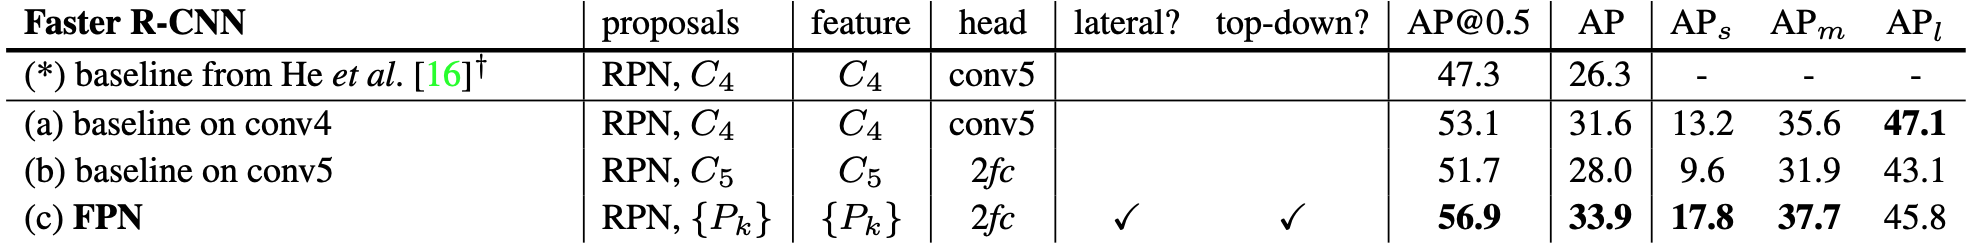
\includegraphics[width=12cm] {images/fpn_results_3}
    %     \caption{Kết quả của thí nghiệm sử dụng kiến trúc FPN cho mô hình Faster R-CNN \index{Faster R-CNN} (Nguồn: \cite{lin2017feature})}
    %     \label{fig:fpn_results_3}
    % \end{figure}

    % \noindent
    % Cụ thể các cấu hình như sau: \\
    % - \textit{baseline from He et al.} là mô hình ResNet được sử dụng cho bài toán nhận diện đối tượng \index{nhận diện đối tượng}. \\
    % - \textit{baseline on conv4} là cấu hình sử dụng feature maps \index{feature maps} từ lớp Conv \index{lớp Conv} thứ 4 của feature extraction module \index{feature extraction module} cho cả hai nhánh của mô hình Faster R-CNN \index{Faster R-CNN}. \\
    % - \textit{baseline on conv5} là cấu hình sử dụng feature maps \index{feature maps} từ lớp Conv \index{lớp Conv} thứ 5 của feature extraction module \index{feature extraction module} cho cả hai nhánh của mô hình Faster R-CNN \index{Faster R-CNN}. \\
    % - \textit{FPN} là cấu hình sử dụng kiến trúc FPN trích xuất feature maps \index{feature maps} cho cả hai nhánh của mô hình Faster R-CNN \index{Faster R-CNN}. \\
    % Trong đó, tất cả các cấu hình được huấn luyện với bộ dữ liệu \textit{COCO trainval135k} và kết quả thu được đánh giá trên bộ dữ liệu \textit{COCO minival}.
    % feature maps \index{feature maps} sử dụng trong cấu hình được ghi chú tại cột \textbf{feature}, kiến trúc mô hình RPN \index{RPN} \cite{ren2015faster} sử dụng trong từng cấu hình được chú thích tại cột \textbf{proposals}, cấu hình của phần head của mô hình Fast R-CNN \index{Fast R-CNN} được chú thích tại cột \textbf{head}, cấu hình có sử dụng lateral connections \index{lateral connections} và top-down pathway hay không được chú thích tại cột \textbf{lateral} và \textbf{top-down}. \\
    % Cấu hình \textit{FPN} đạt kết quả cao hơn vượt trội so với các cấu hình còn lại trên hầu hết các chỉ số đánh giá.
    % Chỉ có duy nhất chỉ số trên đối với các bounding box \index{bounding box} có kích thước lớn thì kết quả của cấu hình \textit{FPN} kém hơn một chút so với cấu hình \textit{baseline on conv4}.

    \noindent
    \textbf{\textit{Vấn đề tồn đọng của kiến trúc mô hình FPN}} \\
    Kiến trúc FPN ra đời đã tạo ra một trong số những kiến trúc backbone \index{backbone} kinh điển trong bài toán nhận diện đối tượng \index{nhận diện đối tượng} nói riêng.
    Kiến trúc FPN đã giúp cho nhiều mô hình đạt độ chính xác cao hơn và trong khi tốc độ của mô hình không bị tăng một cách đáng kể.
    Tuy nhiên, đối với cụ thể bài toán nhận diện đối tượng \index{nhận diện đối tượng}, việc kết hợp kiến trúc FPN vào mô hình Faster R-CNN \index{Faster R-CNN} mới chỉ cải thiện về mặt độ chính xác cho mô hình Faster R-CNN \index{Faster R-CNN} mà chưa giúp tăng tốc mô hình Faster R-CNN \index{Faster R-CNN}.
    Vẫn còn một câu hỏi cần phải được giải quyết đó là làm sao để duy trì được độ chính xác mà FPN mang lại những mô hình nhận diện đối tượng \index{nhận diện đối tượng} vẫn có để đạt tốc độ nhanh hơn nữa.
}
    \fpn

    \subsection{Mô hình RetinaNet}
    \def\retinanet{
    RetinaNet \cite{lin2017focal} là một mô hình single-stage object detection cân bằng giữa độ chính xác của các mô hình two-stage và tốc độ của các mô hình single-stage ở thời điểm đó.
    Nhóm tác giả của RetinaNet đưa ra vấn đề về các mô hình single-stage như YOLO \cite{redmon2016look} hay SSD \cite{liu2016ssd} dù đạt tốc độ rất nhanh nhưng lại kém các mô hình two-stage một khoảng rất xa về độ chính xác và đề xuất giải pháp khắc phục vấn đề này.

    \noindent
    \textbf{\textit{Tổng quan về các mô hình single-stage object detection}} \\
    Các mô hình single-stage object detection ở thời điểm đó đa phần đều chỉ sử dụng một backbone CNN kết hợp thêm với các lớp Conv và lớp fully connected để đưa ra dự đoán về lớp của đối tượng trong ảnh và độ lệch của bounding box so với groundtruth.
    
    \begin{figure}[H]
        \centering
        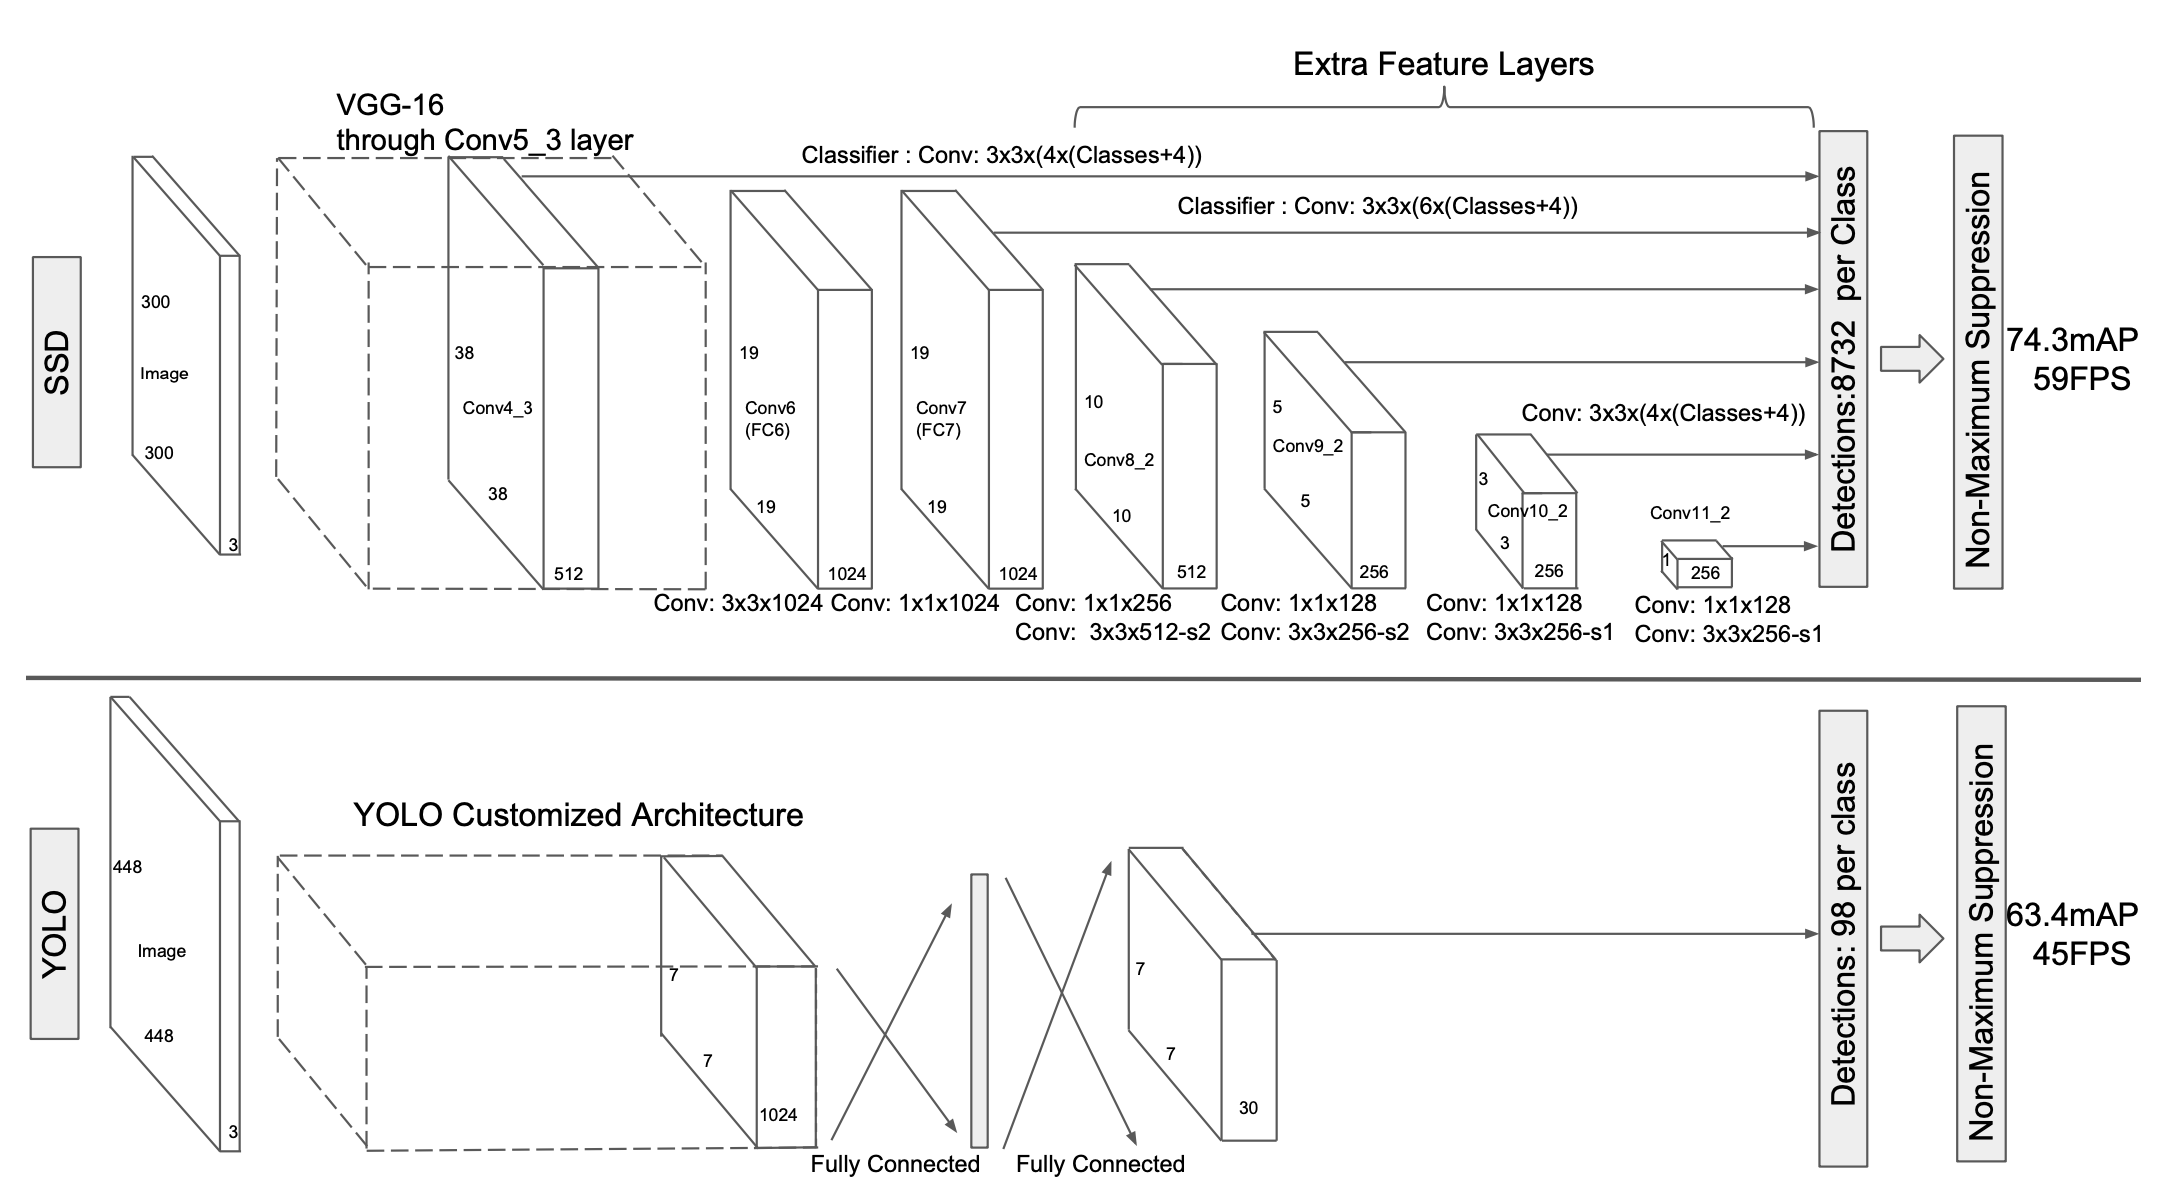
\includegraphics[width=10cm] {images/yolo_ssd_model}
        \caption{Chi tiết hai kiến trúc mô hình single-stage nổi tiếng là SSD và YOLO. (Nguồn: \cite{liu2016ssd})}
        \label{fig:yolo_ssd_model}
    \end{figure}

    \noindent
    Việc loại bỏ Region proposals module khiến các mô hình single-stage object detection cần phải xây dựng một phương pháp riêng nhằm đề xuất ra các anchor chứa đối tượng.
    Hai mô hình single-stage object detection nổi tiếng vào thời điểm đó là YOLO \cite{redmon2016look} và SSD \cite{liu2016ssd} có các cách đề xuất ra anchor tương tự với nhau.
    
    \begin{figure}[H]
        \centering
        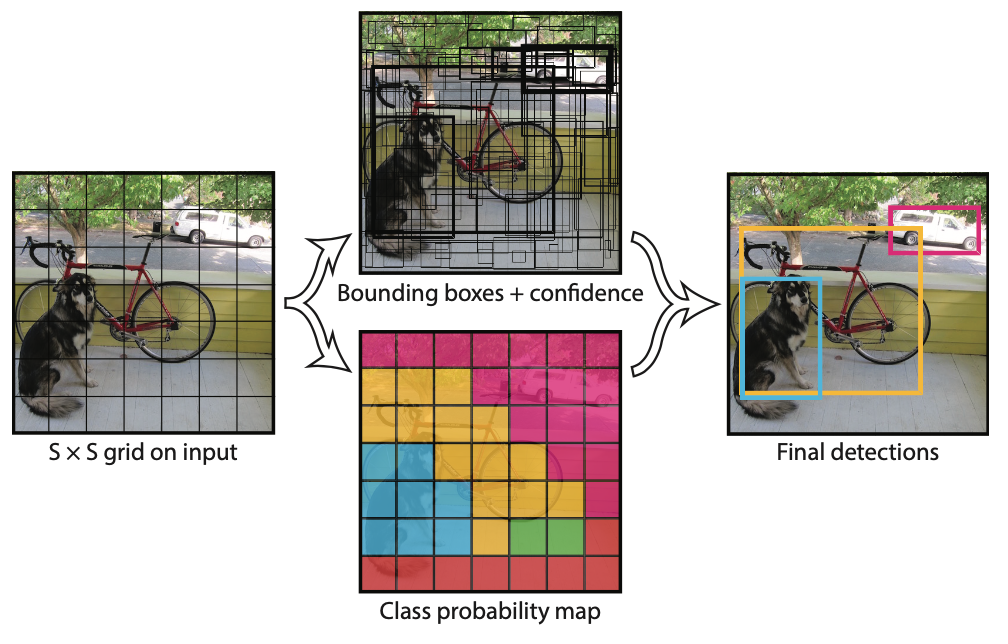
\includegraphics[width=10cm] {images/yolo_anchor}
        \caption{Cách đề xuất anchor của mô hình YOLO. (Nguồn: \cite{redmon2016look})}
        \label{fig:yolo_anchor}
    \end{figure}

    \noindent
    YOLO đề xuất ra các anchor thông qua việc chia ảnh đầu vào thành dạng grid có kích thước $S × S$ và với mỗi grid sẽ trả đầu ra dự đoán có kích thước $S × S × (B * 5 + C)$.
    Nếu tâm của một bounding box nằm trong ô nào trên grid, ô đó sẽ cần phải được dự đoán là chứa đối tượng.
    Mỗi ô trên grid sẽ được mô hình dự đoán $(B * 5 + C)$ giá trị, trong đó: \\
    - B là số lượng bounding box dự đoán. \\
    - 5 là các giá trị trong đó có 4 giá trị x, y, w, h đại diện cho bounding box được dự đoán và 1 giá trị confidence.
    Thay vì được học là 1 nếu anchor có IoU cao với groundtruth bounding box và ngược lại là 0 nếu anchor có IoU thấp với groundtruth bounding box, điểm đặc biệt về giá trị confidence mà nhóm tác giả thiết kế trong mô hình YOLO là nó bằng chính giá trị IoU so với groundtruth. \\
    - C là số lượng lớp đối tượng trong bài toán object detection.
    Mỗi giá trị dự đoán trong C là giá trị xác suất điều kiện nếu ô trên grid chứa đối tượng thì đó là đối tượng nào. \\
    Trong nghiên cứu, nhóm tác giả của YOLO sử dụng $S = 7, B = 2, C = 20$.

    \begin{figure}[H]
        \centering
        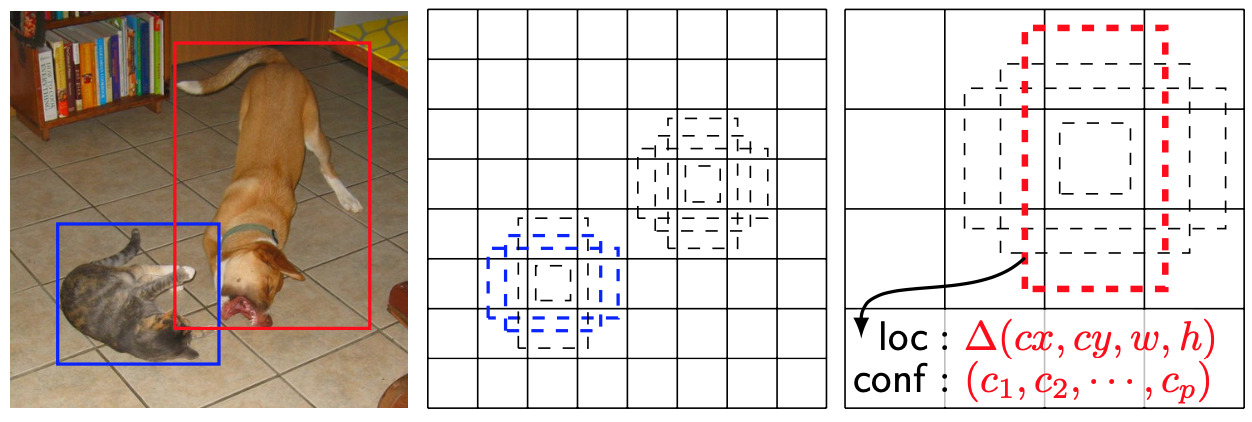
\includegraphics[width=10cm] {images/ssd_anchor}
        \caption{Cách đề xuất anchor của mô hình SSD. (Nguồn: \cite{liu2016ssd})}
        \label{fig:ssd_anchor}
    \end{figure}
    
    \noindent
    SSD cũng sử dụng feature maps như là các dạng grid của ảnh đầu vào nhưng thay vì sử dụng một grid như YOLO thì SSD sử dụng nhiều grid từ nhiều feature maps có cách kích thước khác nhau.
    Với mỗi grid tạo bởi một feature maps có kích thước $m × n$, SSD trả đầu ra dự đoán có kích thước $m × n × (k × (c + 4))$.
    Nếu tâm của một bounding box nằm trong ô nào trên grid, ô đó sẽ cần phải được dự đoán là chứa đối tượng.
    Mỗi ô trên grid sẽ được mô hình dự đoán $(k × (c + 4))$ giá trị, trong đó: \\
    - k là số lượng bounding box dự đoán. \\
    - 4 là 4 giá trị x, y, w, h đại diện cho bounding box được dự đoán. \\
    - c là số lượng lớp đối tượng trong bài toán object detection.
    Mỗi giá trị dự đoán trong c là giá trị xác suất anchor đó là đối tượng nào.

    \noindent
    Với ý tưởng khởi tạo anchor như trên, nhóm tác giả của RetinaNet đã chỉ ra một vấn đề nghiêm trọng mà các mô hình single stage object detection nói chung gặp phải đó là vấn đề mất cân bằng dữ liệu trong quá trình train mô hình.
    Cụ thể, vấn đề mất cân bằng ở đây xảy ra chủ yếu do sự chênh lệch giữa phần ảnh là foreground và phần ảnh là background, hay nói cách khác là phần ảnh chứa đối tượng và phần ảnh không chứa đối tượng. \\
    Các mô hình two-stage object detection không thật sự gặp phải vấn đề mất cân bằng dữ liệu này bởi vì trong quá trình đưa các khu vực đề xuất từ Region proposals module sang Feature extraction module thường đã có một bước lọc và lựa chọn.
    Cụ thể hơn, với số lượng lớn các khu vực không chứa đối tượng được đề xuất bởi Region proposals module, chỉ có một số ít trong đó được lựa chọn để làm đầu vào cho Feature extraction module và lúc này, tỷ lệ giữa các khu vực chứa và không chứa đối tượng thường là 1:3 - một tỷ lệ mất cân bằng không quá nghiêm trọng và không ảnh hưởng tới việc train mô hình object detection.

    \noindent
    \textbf{\textit{Hàm Focal loss}} \\
    Để giải quyết vấn đề mất cân bằng dữ liệu nói trên, nhóm tác giả của RetinaNet đã đề xuất hàm Focal loss dựa trên nền tảng của hàm binary cross entropy loss giải quyết vấn đề mất cân bằng dữ liệu nghiêm trọng.
    Nhóm tác giả chú thích rằng hàm Focal loss hiệu quả đối với cả bài toán phân lớp với nhiều hơn hai lớp nhưng để đơn giản hoá, nhóm tác giả sử dụng hàm binary cross entropy loss.

    \begin{equation}
        \label{eq:bce}
        CE(p,y) = 
        \begin{cases}
            -\log(p) &\text{if $y = 1$} \\
            -\log (1 - p) &\text{otherwise.}
        \end{cases}
    \end{equation}

    \noindent
    trong đó: \\
    - y là giá trị groundtruth (0 đối với anchor không chứa object và 1 đối với anchor chứa object) \\
    - p là giá trị xác suất mà mô hình dự đoán anchor đó chứa object \\
    Để ngắn gọn, nhóm tác giả quy ước lại như sau:

    \begin{equation}
        \label{eq:bce}
        p_\textrm{t} =
        \begin{cases}
            p &\text{if $y = 1$} \\
            1 - p &\text{otherwise,}
        \end{cases}
    \end{equation}

    \noindent
    từ đó, hàm cross entropy loss được viết lại thành

    \begin{equation}
        CE(p,y) = CE(p_\textrm{t}) = - \log (p_\textrm{t})
    \end{equation}

    \noindent
    Một cấu hình khác của hàm cross entropy loss là \textit{balanced cross entropy loss}, được sinh ra bằng việc đánh trọng số cho từng số hạng của hàm cross entropy loss ban đầu

    \begin{equation}
        CE(p,y) = - \alpha_\textrm{t} \log (p_\textrm{t})
    \end{equation}

    \noindent
    trong đó: \\
    - $\alpha_\textrm{t}$ là trọng số tương ứng với số hạng $p_\textrm{t}$.
    Trọng số $\alpha_\textrm{t}$ có thể được tính dựa trên tần suất xuất hiện của các lớp trong bộ dữ liệu hoặc là một hyperpameter.

    \noindent
    Hàm balanced cross entropy loss có thể đã giúp giảm bớt hiệu ứng mất cân bằng dữ liệu lên trên giá trị hàm loss.
    Tuy nhiên, việc gán trọng số như hàm balanced cross entropy loss không phân biệt được giữa những mẫu dữ liệu dễ và khó.
    Nhóm tác giả, từ đó, đề xuất hàm \textit{Focal loss} không những giúp giải quyết vấn đề mất cân bằng dữ liệu mà còn giúp mô hình tập trung vào những mẫu dữ liệu \textit{không chứa đối tượng} nhưng khó và dễ nhầm lẫn thành \textit{chứa đối tượng}.

    \begin{equation}
        FL(p_\textrm{t}) = - (1 - p_\textrm{t})^\gamma \log (p_\textrm{t})
    \end{equation}

    \noindent
    trong đó: \\
    - $(1 - p_\textrm{t})$ là thành phần đánh giá độ dễ hay khó của mẫu dữ liệu.
    Với những mẫu dễ và mô hình đã được train tốt, giá trị $(1 - p_\textrm{t})$ sẽ nhỏ và những mẫu này sẽ gây ít ảnh hưởng trong quá trình train mô hình. \\
    - $\gamma$ được nhóm tác giả gọi là \textit{focusing parameter}, dùng để xác định mức độ tập trung của mô hình lên các mẫu dữ liệu không chứa đối tượng.
    Với $\gamma = 0$, hàm FL lúc này tương tự với hàm CE.
    Trong các thí nghiệm của RetinaNet, giá trị $\gamma = 2$ là tốt nhất.

    \begin{figure}[H]
        \centering
        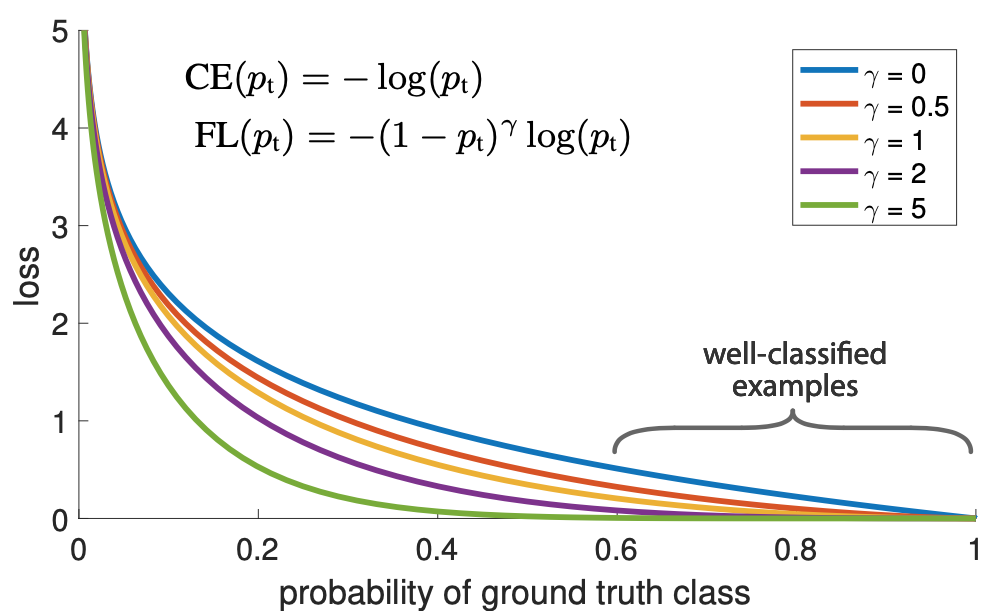
\includegraphics[width=10cm] {images/retinanet_focal_loss_curve}
        \caption{So sánh các tham số của hàm Focal loss với hàm Cross Entropy loss. (Nguồn: \cite{lin2017focal})}
        \label{fig:retinanet_focal_loss_curve}
    \end{figure}

    \noindent
    Ngoài ra, nhóm tác giả còn đề xuất một dạng khác của hàm FL bằng việc sử dụng thêm một tham số $\alpha$ và trong các thí nghiệm, dạng này cho kết quả tốt hơn một chút so với dạng hàm FL không sử dụng $\alpha$.

    \begin{equation}
        FL(p_\textrm{t}) = - \alpha_\textrm{t} (1 - p_\textrm{t})^\gamma \log (p_\textrm{t})
    \end{equation}
    
    \noindent
    \textbf{\textit{Kiến trúc mô hình RetinaNet}} \\
    RetinaNet là mô hình single-stage object detection gồm có các thành phần:
    - Phần \textit{backbone Feature Pyramid Networks} được sử dụng nhằm trích xuất đặc trưng của ảnh đầu vào với nhiều kích thước đặc trưng khác nhau.
    Chi tiết về sức mạnh của FPN đã được thảo luận ở \textit{phần 2.2. Kiến trúc Feature Pyramid Networks}.
    - Phần trích xuất anchor được thực hiện tương tự với cách trích xuất của mô hình RPN biến thể đã phân tích ở \textit{phần 2.2}.
    Tuy nhiên, nhóm tác giả đã thử nghiệm và bổ sung thêm các kích thước $2^{0}$, $2^{1/3}$, $2^{2/3}$ của anchor để đạt kết quả tốt hơn.
    Các anchor được gán groundtruth với chiến lược tương tự như trong \textit{phần 2.1.3. Mô hình Faster R-CNN} nhưng điều chỉnh một số điểm: (1) thay đổi trở thành bài toán multi-class classification (nhóm tác giả của \textit{phần 2.1.3} sử dụng bài toán binary classification phân lớp giữa \textit{anchor có chứa object} và \textit{anchor không chứa object}) và (2) thay đổi threshold IoU để gán nhãn cho từng anchor.

    \begin{figure}[H]
        \centering
        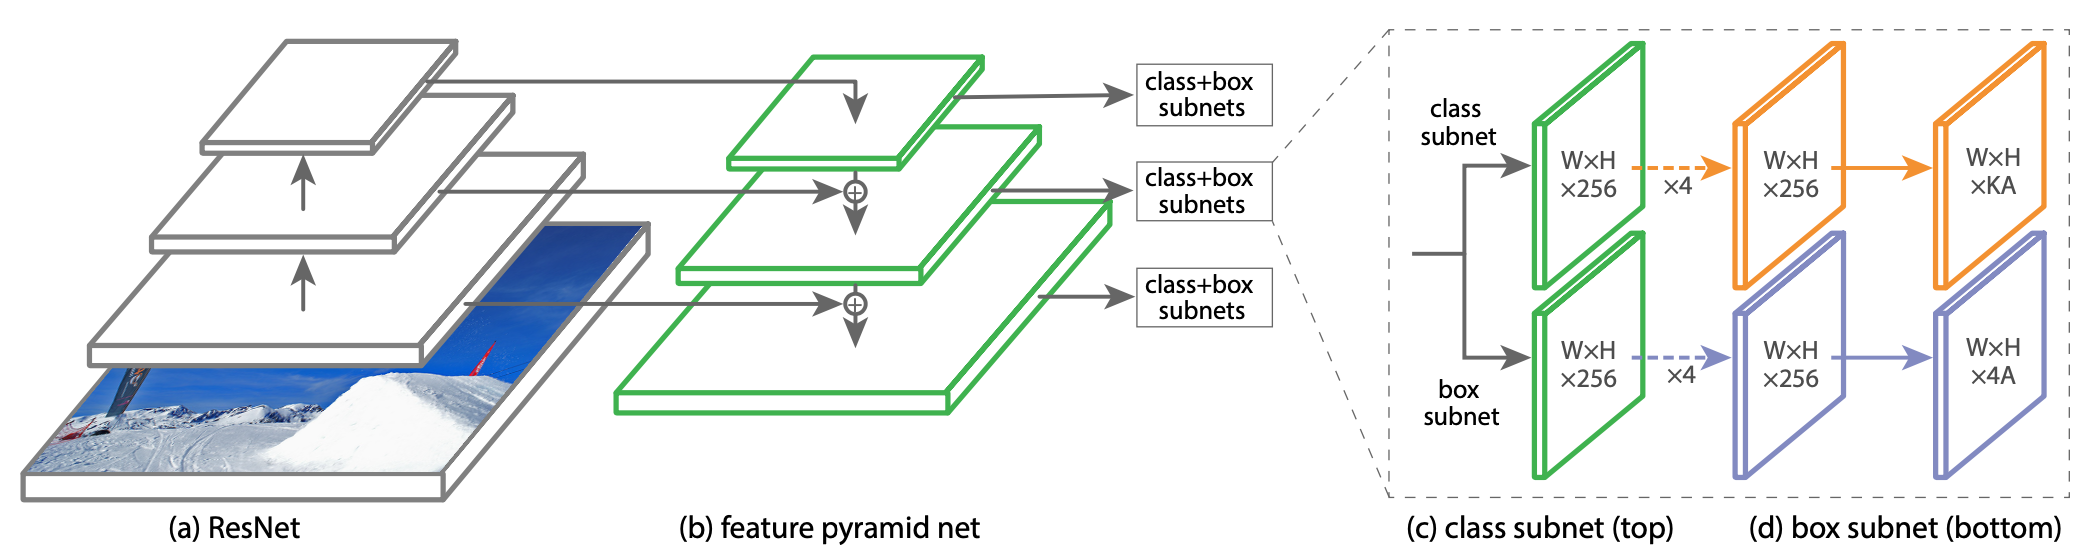
\includegraphics[width=10cm] {images/retinanet_model}
        \caption{Kiến trúc mô hình RetinaNet. (Nguồn: \cite{lin2017focal})}
        \label{fig:retinanet_model}
    \end{figure}

    \noindent
    - Phần \textit{Classification Subnet} được chia sẻ giữa tất cả các feature maps của backbone FPN, gồm các lớp Conv 3x3xC và lớp Conv cuối cùng 3x3xKA.
    Trong đó, K là số lượng lớp đối tượng trong bài toán object detection, A là số lượng anchor tại vị trí trên mỗi feature maps của backbone FPN (tác giả chọn $A = 9$), C là số lượng channel của lớp Conv (tác giả chọn $C = 256$). \\
    - Phần \textit{Box Regression Subnet} được thiết kế khác với cách thiết kế trong mô hình Faster R-CNN khi không dùng chung các lớp Conv với \textit{Classification Subnet}.
    \textit{Box Regression Subnet} cũng gồm các lớp Conv 3x3xC và lớp Conv cuối cùng 3x3x4A.
    Trong đó, A là số lượng anchor tại vị trí trên mỗi feature maps của backbone FPN (tác giả chọn $A = 9$), 4 là 4 độ lệch trong toạ độ của bounding box dự đoán so với groundtruth, C là số lượng channel của lớp Conv (tác giả chọn $C = 256$).

    \noindent
    \textbf{\textit{Kết quả của mô hình RetinaNet}} \\
    Trong thử nghiệm của RetinaNet với các tham số khác nhau của hàm Focal loss, tất cả các cấu hình được train với bộ dữ liệu \textit{COCO trainval135k} và kết quả thu được đánh giá trên bộ dữ liệu \textit{COCO minival}.
    Kết quả của cấu hình $\gamma = 2.0$ và $\alpha = 0.25$ đạt kết quả tốt nhất so với các cấu hình khác của hàm Focal loss.

    \begin{figure}[H]
        \centering
        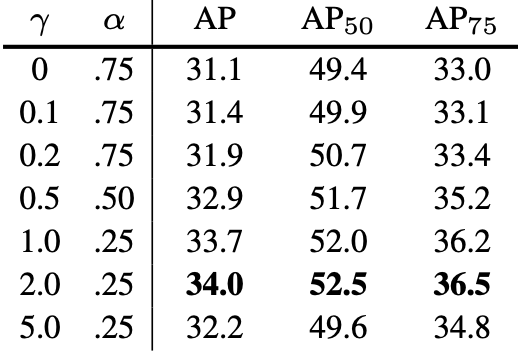
\includegraphics[width=10cm] {images/retinanet_results_2}
        \caption{Kết quả thử nghiệm hàm Focal loss với các tham số khác nhau. (Nguồn: \cite{lin2017focal})}
        \label{fig:retinanet_results_2}
    \end{figure}

    Khi so sánh kết quả của mô hình RetinaNet với các mô hình object detection khác vào thời điểm đó, kết quả của các cấu hình khác nhau của mô hình RetinaNet cũng đạt kết quả rất tốt về cả tốc độ lẫn độ chính xác của mô hình.
    Cụ thể các mô hình được so sánh gồm: \\
    - Kết quả của mô hình YOLOv2 ký hiệu là [A] \cite{redmon2016yolo9000} (Kết quả không được biểu diễn trên hình) \\
    - Kết quả của mô hình SSD321, ký hiệu là [B] \cite{liu2016ssd} \\
    - Kết quả của mô hình DSSD321, ký hiệu là [C] \cite{fu2017dssd} \\
    - Kết quả của mô hình R-FCN, ký hiệu là [D] \cite{dai2016r} \\
    - Kết quả của mô hình SSD513, ký hiệu là [E] \cite{liu2016ssd} \\
    - Kết quả của mô hình DSSD513, ký hiệu là [F] \cite{fu2017dssd} \\
    - Kết quả của mô hình FPN FRCN, ký hiệu là [G] \cite{lin2017feature} \\
    - Kết quả của mô hình RetinaNet sử dụng backbone là ResNet50 và sử dụng ảnh đầu vào có kích thước 500 pixel, ký hiệu là RetinaNet-50-500. \\
    - Kết quả của mô hình RetinaNet sử dụng backbone là ResNet101 và sử dụng ảnh đầu vào có kích thước 500 pixel, ký hiệu là RetinaNet-101-500 \\
    - Kết quả của mô hình RetinaNet sử dụng backbone là ResNet101 và sử dụng ảnh đầu vào có kích thước 800 pixel, ký hiệu là RetinaNet-101-800 \\
    Đường màu xanh và màu cam trên hình lần lượt là các cấu hình RetinaNet sử dụng backbone ResNet50 và ResNet101 và với các cấu hình ảnh đầu vào từ 400 pixel đến 800 pixel.

    \begin{figure}[H]
        \centering
        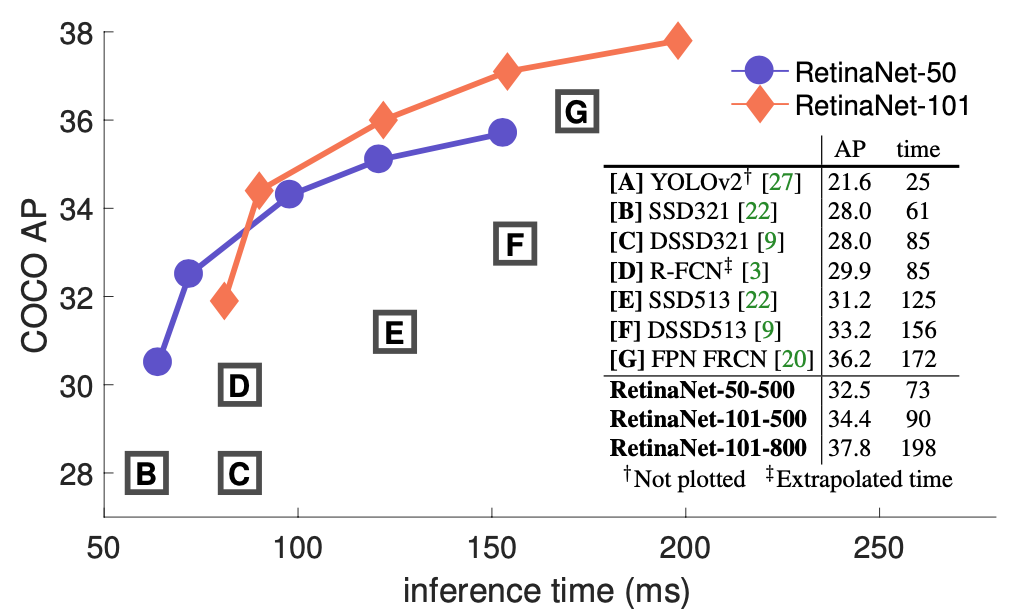
\includegraphics[width=6cm] {images/retinanet_results_1}
        \caption{So sánh kết quả mô hình RetinaNet với một số mô hình object detection khác. (Nguồn: \cite{lin2017focal})}
        \label{fig:retinanet_results_1}
    \end{figure}

    Kết quả, các cấu hình khác nhau của RetinaNet đều cho kết quả tốt hơn so với các mô hình object detection khác (cả single-stage và two-stage).
    So với mô hình đạt độ chính xác tốt nhất ở thời điểm đó là [G], cấu hình RetinaNet-101-700 cho kết quả chính xác hơn với thời gian nhanh hơn.
    So với các mô hình đạt tốc độ tốt nhất ở thời điểm đó là [A] và [B], cấu hình RetinaNet-50-400 cho kết quả chậm hơn nhưng với độ chính xác cao hơn vượt trội.

    \noindent
    \textbf{\textit{Kết luận về mô hình RetinaNet}} \\
    Mô hình RetinaNet ra đời là một bước tiến lớn đối với việc giải quyết bài toán object detection khi nó giải quyết vấn đề mất cân bằng dữ liệu của các mô hình single-stage giúp tăng độ chính xác của mô hình ngang bằng với các mô hình two-stage nhưng vẫn duy trì được một tốc độ nhanh và có thể sử dụng trong thời gian thực. \\
    Mô hình RetinaNet cho đến nay vẫn là một mô hình tốt để giải quyết các bài toán con của object detection, cụ thể là face detection.
    Trong các phần tiếp theo của luận văn, ta sẽ bàn luận về các mô hình kế thừa RetinaNet giải quyết rất tốt bài toán face detection.
}
    \retinanet
}